\documentclass{article}
\usepackage{graphicx} 
\usepackage{amsmath, amsfonts, amssymb, amsthm}
\usepackage{tikz}
\usepackage{float}

\usetikzlibrary{graphs}
\usepackage[demo]{graphicx}
\usepackage{subfig}

% just took these from the presentation. might have some errors, idk how this stuff works
\usepackage{tikz}
\usepackage{pgfplots}
\pgfplotsset{compat = newest}
\usetikzlibrary{matrix}
\usepackage[dvipsnames]{xcolor}
\usetikzlibrary{perspective}


% copypasted from 
% https://www.dickimawbooks.com/latex/thesis/html/amsthm.html
\theoremstyle{plain}
\newtheorem{theorem}{Theorem}
\newtheorem{lemma}{Lemma}

\theoremstyle{definition}
\newtheorem{defn}{Definition}
\newtheorem{conj}{Conjecture}

\theoremstyle{remark}
\newtheorem*{note}{Note}
\newtheorem{remark}{Remark}


\usepackage{verbatim}
\usepackage{tabularx}
\usepackage{indentfirst} % Indent first paragraph in each section
\usepackage[a4paper, total={6in, 8.1in}]{geometry}
\usepackage{setspace}


\newcommand{\mat}{\text{Mat}}
\newcommand{\cl}{\mathrm{cl}}
\newcommand{\caf}{\mathcal{F}}
\newcommand{\rank}{\text{r}}

\onehalfspacing

% Equations should be numbered per section
\numberwithin{equation}{section}

\title{Cryptomorphic Descriptions of Matroids}
\author{Adriel Matei, Béla Schneider, Javier Vela Castro, Juš Kocutar}

\begin{document}

\maketitle

\section{Introduction}
\subsection{(In)dependence}

In english language, two peolpe, objects or concepts are dependent on each other if both in some way influence one another. Two things being independent from each other then means that they in no way can affect eachother. 

In mathematics there are many concepts where we can use these two words to describe certain phenomena, most notably, linear algebra. In linear algebra, a set of vectors is linearly dependent if you can write one of its vectors as a linear combination of the others. Using the word dependent here makes sense, because if you can use all others to build that one vector, then that vertor does not really stand on its own. An equivalent and more general definition is:
$$ \{v_1,v_2,\dots,v_n\} \text{ is linearly dependent if} $$ $$ \text{there exists } a_1,a_2,\dots,a_n \in \mathbb{R} \text{ not all zero, such that } a_1v_1+a_2v_2+\dots +a_nv_n = 0$$
For linear independence we have the negation, which is:
$$ \{v_1,v_2,\dots,v_n\} \text{ is linearly independent if } $$ $$ a_1v_1+a_2v_2+\dots+a_nv_n=0 \text{ implies that } a_1=a_2=\dots=a_n=0 $$

There are many more fields that have this concept of (in)dependence present in some way. To relate these with another we will abstract the concept of (in)dependence into mere sets that follow certain rules. It turns out that by doing this we can find independence in places that do not even use the terms (in)dependence, most notably, graph theory.

%TODO: give an intuitive explaination on why cycles in graphs are somehow 'dependent'





\newpage

\subsection{Matroids}

A matroid is a structure that abstracts the notion of independence. To construct a matroid we first start with a ground set that is finite. We do not want to work with infinite sets, because that causes lots of problems. Next, we construct a set of subsets of the ground set, following a couple of rules. Usually, this would be the set of independent sets. However, it turns out that there are many surprisingly equivalent (cryptomorphic) ways of defining a matroid, such as:
\begin{itemize}
    \item Independent sets
    \item Bases
    \item Circuits
    \item Rank function
    \item Closure operator
    \item Flats
\end{itemize}

There are many more cryptomorphic ways to define a matroid, but the ones listed will be covered in this article. Each of these mathematical objects has two to four axioms that uniquely determine it as the object characterizing a matroid. To show the cryptomorphism, we will have to prove a certain equivalence each time. All of this will help us gain a deeper insight into the concept of dependence and independence.

\section{Definitions}
\newpage
\section{Elementary Definitions}

\subsection{Independent sets}

We will begin with the first possible way of defining what a \textit{matroid} is. This way is arguably the simplest one because the properties are intuitive and not hard to visualize. When speaking about matroids, we will always deal with finite sets, and the way we obtain a matroid from a finite set is to select some special selection of its subsets.  These special sets correspond to the \textit{independent} sets, and should obey some distinctive properties. This idea is precisely what the following definition is about.

\begin{defn}
    Let $E$ be a finite set, possibly empty, and $\mathcal{I}$ a collection of subsets of $E$ (i.e. some subset of the power set $2^E$ of E). We call the ordered pair $M = (E, \mathcal{I})$ a matroid if the following three properties are satisfied

    \begin{enumerate}
        \item[(I1)] We have $\emptyset \in \mathcal{I}$.
        
        \item[(I2)] If $I \in \mathcal{I}$ and $J \subseteq I$, then $J \in \mathcal{I}$.
        
        \item[(I3)] If $J, I \in \mathcal{I}$ and $|J| < |I|$, then there exists $e \in I - J$ so that $J \cup e \in \mathcal{I}$.
    \end{enumerate}

    We call elements of $\mathcal{I}$ \textbf{independent sets}. 
\end{defn}

There are some alternatives to the third property that are equivalent, for example we could alternatively write

\begin{enumerate}
    % The `\ ` is the hackiest thing ever, please ignore it :/
    \item [(3.*)$\ $] \textit{ If $I, J \in \mathcal{I} $ and $|J| = |I| + 1$, then there exists $e \in J - I$ such that $I \cup e \in \mathcal{I}$.}
\end{enumerate}

or

\begin{enumerate}
\item[(3.**)] \textit{If $X \subseteq E$ and $I_1, I_2$ are maximal members of $\{ I \in \mathcal{I} | I \subseteq X \}$, then $|I_1| = |I_2|$.}
\end{enumerate}

\begin{exmp}
In  figure (\ref{fig:1234-matroid-independent-sets}) we find a representation of a matroid by writing all subsets of the ground set $\{1,2,3,4\}$ and coloring them accordingly. The independent sets are colored in orange. It is clear that the empty set is independent and that all subsets of independent sets are independent. The dependent sets, colored in cyan, are the sets that are not independent.
\end{exmp}


\begin{figure}[h]

\begin{center}
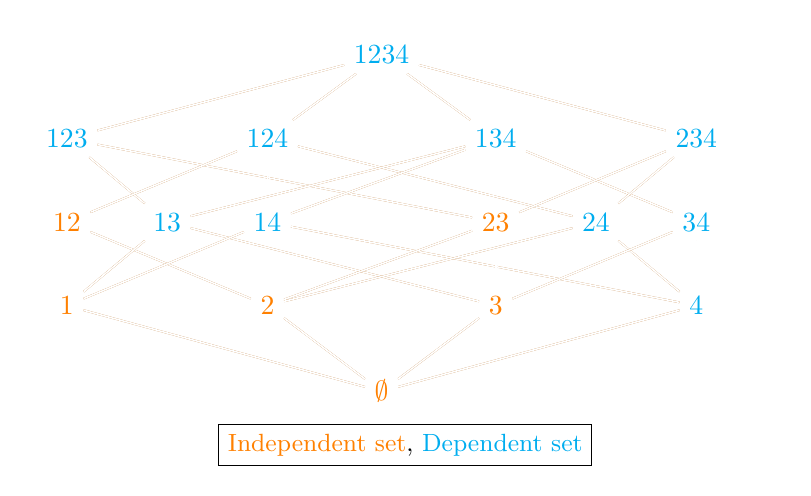
\begin{tikzpicture}

\matrix (a) [matrix of math nodes, column sep=0.6cm, row sep=0.6cm,]{
 & & &\textcolor{cyan}{
1234} & & & &\\
 \textcolor{cyan}{
123}& &\textcolor{cyan}{
124} & &\textcolor{cyan}{
134} &  & \textcolor{cyan}{
234}  \\
\textcolor{orange}{12} & \textcolor{cyan}{13} & \textcolor{cyan}{14} & & \textcolor{orange}{23} & \textcolor{cyan}{
24} & \textcolor{cyan}{
34} \\
\textcolor{orange}{1}& &\textcolor{orange}{2} & & \textcolor{orange}{3}& & \textcolor{cyan}{4} \\
& & & \textcolor{orange}{\emptyset} &  & & \\
&&&&&& \\};

\foreach \i/\j in {1-4/2-1, 1-4/2-3, 1-4/2-5, 1-4/2-7, 2-1/3-1, 2-1/3-2, 2-1/3-5, 2-3/3-1, 2-3/3-3, 2-3/3-6, 2-5/3-2, 2-5/3-3, 2-5/3-7, 2-7/3-5, 2-7/3-6, 2-7/3-7, 3-1/4-1, 3-1/4-3, 3-2/4-1, 3-2/4-5, 3-3/4-1, 3-3/4-7, 3-5/4-3, 3-5/4-5, 3-6/4-3, 3-6/4-7, 3-7/4-7, 3-7/4-5, 4-1/5-4, 4-3/5-4, 4-5/5-4, 4-7/5-4}
\draw[double, line width = 0.005mm, color = brown] (a-\i) -- (a-\j);

\node[draw] at (0, -2.5){\small \textcolor{orange}{Independent set}, \textcolor{cyan}{Dependent set}};

\end{tikzpicture} % why does it say this??? Did you forget a semicolon?
\end{center}
\caption{Diagram of a 4-element matroid, with dependent and independent sets colored accordingly.}
\label{fig:1234-matroid-independent-sets}
\end{figure}


The definition of a matroid is designed to extract out the property that makes a subset of elements 'independent'. This leads us to our first examples, namely the so-called \textit{representable matroids} arising from linear algebra. We say that a subset of vectors is \textit{independent} in a matroid, if and only if it is \textit{linearly independent} in the usual sense. 
%This means, in particular, that the subsets have the same properties.



 Let $A \in \mat_{m \times n}(\mathbb{F})$ where $\mathbb{F}$ is a field. In the article we will not just be interested with $\mathbb{F} = \mathbb{C} \; \mathrm{or}\; \mathbb{F} = \mathbb{R} $ but also in finite fields\footnote{In particular, we are interested in $\mathbb{Z} / p\mathbb{Z}$. By that we mean $\mathbb{Z}$ modulo $p\mathbb{Z}$ so the set of reminders when dividing by a prime number $p$. We will denote this field by $\mathbb{F}_p$}.

\begin{exmp}
    

 
 We will pick a concrete example of $A \in  \mat_{3 \times 4}(\mathbb{R})$ to illustrate that the set of columns of a matrix has a natural matroid structure. Suppose

$$A = \begin{pmatrix}

2 & 0 & 2 & 0 \\
1 & -1 & 0 & 0 \\
0 & 3 & 3 & 0


\end{pmatrix}.$$

We would like to consider \textit{the set of labels of columns of the matrix $A$} and form a matroid on it. This means we start with $E = \{1,2,3,4\}$ so a finite set where the number $1$ corresponds to the column $\begin{pmatrix} 2 & 1 & 0 \end{pmatrix} ^ T$, the number 2 corresponds to $\begin{pmatrix}  0 & -1 & 3  \end{pmatrix} ^ T$ and so forth. We now declare that a subset of $E$ is called independent if and only if the corresponding set of column vectors is linearly independent as a set of vectors in $\mathbb{R}^3$. We can explicitly check what this means in our example. The sets $\{1\}$, $\{2\}$, $\{3\}$ are all independent because they correspond to non-zero vectors. For the two-element subsets we see that $\{1,2\}$, $\{1,3\}$ and $\{2,3\}$ are all independent, while any two element subsets containing the last column are not. Finally, the 3-element subset $\{1,2,3\}$ is not independent because as vectors, the first and the second column sum up to the third. So to conclude, the collection of all independent sets is
$$\mathcal{I} = \{\emptyset, \{1\}, \{2\}, \{3\}, \{1,2\}, \{1,3\}, \{2,3\} \},$$

which indeed satisfies the properties of collection of independent sets of a matroid. This is not a coincidence, we will prove that a collection of subsets formed from a matrix in the above way is always a matroid.

\end{exmp}


\begin{theorem}

    Let $A \in \mathrm{Mat} _{m \times n}(\mathbb{F})$ and $E = \{1, 2, \cdots, n\}$ be a finite set of $n$ elements where the element $i$ corresponds to the $i$-th column of the matrix $A$. We call a subset $I \subseteq E$ independent if and only if the column vectors that the members of $I$ correspond to form a linearly independent set as members of $\mathbb{F}^n$, and denote the collection of all independent subsets as $\mathcal{I}$. Then $M = (M, \mathcal{I})$ is a matroid, and we denote it by $M[A]$.
    
\end{theorem}

\begin{proof}
    The idea of the proof is taken from \cite[p. 8]{oxley1}.
    We need to check that the collection $\mathcal{I}$ satisfies the three properties for the collection of independent sets given in the definition. 

\begin{enumerate}

    \item[(I1)] First, $\emptyset$ is trivially in $\mathcal{I}$.
    
    \item[(I2)] The second property is also satisfied because if $J \subseteq I$ and $I \in \mathcal{I}$ this means that the vectors corresponding to $I$ form a linearly independent set. In particular, let $v_1, v_2, \cdots v_j, v_{j+1}, \cdots v_{i}$ be the column vectors corresponding to $I$, and that first $j$ are also in $J$, that means $|I| = i$, $|J| = j$ and $j \leq i$. If for some linear combination we have $a_1v_1 + \cdots + a_jv_j = 0$, where $a_i \in \mathbb{F}$ then it is also true that $a_1v_1 + \cdots + a_jv_j + 0 \cdot a_{j+1} + \cdots + 0 \cdot a_i = 0$. Since the vectors of $I$ are linearly independent it now follows that $a_1 = a_2 = \cdots a_j = 0$ as well. So the vectors corresponding to the elements of $J$ are also linearly independent, which means by definition $J \in \mathcal{I}$.

    \item[(I3)] Finally, we have to check third property. We assume that $J, I \in \mathcal{I}$ and $|J| < |I|$. We denote by $V_J$ and $V_I$ the linear subspaces of $\mathbb{F}^n$ spanned by vectors corresponding to $J$ and $I$ respectively. Because the vectors corresponding to $J$ and $I$ are linearly independent, they also form a basis for $V_J$ and $V_I$ respectively. For any $e \in I - J$ we denote by $v(e) \in \mathbb{F}^n$ the column vector of $A$ corresponding to $e$. Suppose some $e \in I - J$ has the property that adding it to $J$ does not change the dimension of the subspace spanned by J, i.e. $\dim (V_J \cup v(e)) = \dim (V_J) = |J|$. Then $v(e)$ is already in $V(J)$ because the vectors corresponding to $J$ are linearly independent and if the dimension does not increase, then $v(e)$ can be expressed as a linear combination of vectors corresponding to $J$. However, this cannot hold true for \textit{every} $e \in I - J$. Suppose for contradiction, that for every $e \in I - J$ it holds that the vector $v(e) $ is already in $ V_J$. Because for all elements in the intersection,  $i \in I \cap J$, we have $v(i) \in V_J$ by definition, we could then infer $V_I \subseteq V_J$. But this implies that 

    $$|I| = \dim(V_I) = \dim(V_J) = |J| < |I|$$
     which is a contradiction. So there is at least one $e \in I - J$ so that $\dim(V_J \cup v(e)) = \dim(V_J) + 1$, which means the vectors corresponding to $J \cup e$ form a linearly independent subset. Finally, this means that $J \cup e \in \mathcal{I}$ which proves the third property.

\end{enumerate}
\end{proof}

In order to talk about any classification of matroids we have to say when the two matroids are equivalent - representing the same structure of independent sets. Intuitively, it is nothing deep, the definition will just rephrase that the two are \textit{equal} if it is possible to relabel the elements of the first matroid to the elements of the second without changing the independent sets.

\begin{defn}
    We call two matroids $M = (E, \mathcal{I})$ and $N = (F, \mathcal{J})$ isomorphic and denote it by $M \sim N$ if there exists a bijection $f: E \to F$ so that a subset $K \subseteq F$ is independent if and only if $K = f(L)$ for some independent set $L \in \mathcal{I}$.
\end{defn}


\begin{defn}
    We call a matroid $M$ representable, if $M$ is isomorphic to a matrix matroid $N[A]$ for some $A \in \mat_{m \times n}(\mathbb{F})$ over some field $\mathbb{F}$. Moreover, we  call it $\mathbb{F}$-representable if it is representable over specific field $\mathbb{F}$.
\end{defn}

We will now define another important class of matroids. Due to its simplicity it will be suitable as an example in many of the notions defined in the proceeding text.

\begin{defn}\label{uniformM}
    Let $E = \{1, 2, \cdots, n\}$ and $\mathcal{I} = \{ L \subseteq E \; \text{ such that } \; |L| \leq m\}$. Then $(E, \mathcal{I})$ is a matroid which we denote by $U_{m,n}$ and call it a uniform matroid of rank $m$ on a $n$ element set.
\end{defn}
\begin{theorem}
    The ordered pair $U_{m,n} = (E, \mathcal{I})$ is a matroid.
\end{theorem}

\begin{proof}
    
It is easy to check that $U_{m,n}$ is indeed a matroid. 

\begin{enumerate}
   

    \item[(I1)] For any $m \geq 0$ we have $\emptyset \in \mathcal{I}$ since $|\emptyset | = 0$.
    \item[(I2)] If $I \in \mathcal{I}$ and $J \subseteq I$ then $|J|\leq |I|$ so $|J|\leq |I| \leq m$ implying $J \in \mathcal{I}$ by definition.
    \item[(I3)] Finally, if $I, J \in \mathcal{I}$ and $|J|<|I|$ then for any $e \in I - J$ we will have $|J \cup e| = |J| + 1 \leq |I| \leq m$ so $J \cup e \in \mathcal{I}$ by definition for any $e \in I - J.$


\end{enumerate}
\end{proof}

\subsection{Bases}

Let $M = (E, \mathcal{I})$ be a matroid. We call a subset $B \subseteq E$ a \textit{basis} if it is a \textit{maximal independent set}. That means that $B$ is an independent set and $B$ is not properly contained inside any other independent set. It turns out that bases for matroids and bases for vector subspaces have some similarities in their properties. In particular the third property of independent sets immedietly guarantees us that all matroid bases have the same size, just like vector bases for finite-dimensional vector spaces.

\begin{theorem} \label{thm:bases-have-equal-size}
    Let $M = (E, \mathcal{I})$ be a matroid. Then all bases of $M$ have the same size.
\end{theorem}

\begin{proof}
    Aiming for contradiction, suppose that the theorem does not hold. Let $B$ and $S$ be two bases with $|B| < |S|$ - different size. By the third property of independent sets we know there exists $e \in S - B$ such that $ B \cup e \in \mathcal{I}$. However, then $B$ is properly contained inside $B \cup e$, another independent set, which contradicts its maximality. So the initial assumption that there exist two bases with different size is false.
\end{proof}

The concept of a basis is important because it allows us to define a \textit{rank function} of a matroid, which computes the size of the maximal independent subset inside a given subset of a matroid.  Because the sizes of all of such sets --- bases --- are equal, this will be a well-defined notion.

\begin{exmp}
    In figure (\ref{fig:1234-matroid-bases}), we find a depiction of the same matroid from figure (\ref{fig:1234-matroid-independent-sets}). In addition, we also highlight the bases of the matroid in red. Two properties can be observed:
\begin{enumerate}
    \item The bases are the maximally independent subsets, which means that all of their proper supersets are dependent. 
    \item Both bases contain two elements (they have the same size).
\end{enumerate}
\end{exmp}

\begin{figure}[h]

\begin{center}
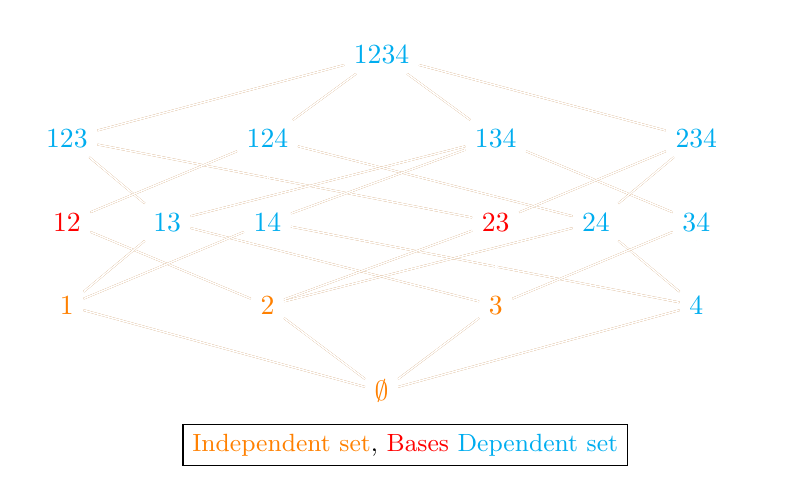
\begin{tikzpicture}

\matrix (a) [matrix of math nodes, column sep=0.6cm, row sep=0.6cm,]{
 & & &\textcolor{cyan}{
1234} & & & &\\
 \textcolor{cyan}{
123}& &\textcolor{cyan}{
124} & &\textcolor{cyan}{
134} &  & \textcolor{cyan}{
234}  \\
\textcolor{red}{12} & \textcolor{cyan}{13} & \textcolor{cyan}{14} & & \textcolor{red}{23} & \textcolor{cyan}{
24} & \textcolor{cyan}{
34} \\
\textcolor{orange}{1}& &\textcolor{orange}{2} & & \textcolor{orange}{3}& & \textcolor{cyan}{4} \\
& & & \textcolor{orange}{\emptyset} &  & & \\
&&&&&& \\};

\foreach \i/\j in {1-4/2-1, 1-4/2-3, 1-4/2-5, 1-4/2-7, 2-1/3-1, 2-1/3-2, 2-1/3-5, 2-3/3-1, 2-3/3-3, 2-3/3-6, 2-5/3-2, 2-5/3-3, 2-5/3-7, 2-7/3-5, 2-7/3-6, 2-7/3-7, 3-1/4-1, 3-1/4-3, 3-2/4-1, 3-2/4-5, 3-3/4-1, 3-3/4-7, 3-5/4-3, 3-5/4-5, 3-6/4-3, 3-6/4-7, 3-7/4-7, 3-7/4-5, 4-1/5-4, 4-3/5-4, 4-5/5-4, 4-7/5-4}
\draw[double, line width = 0.005mm, color = brown] (a-\i) -- (a-\j);

\node[draw] at (0, -2.5){\small \textcolor{orange}{Independent set}, \textcolor{red}{Bases} \textcolor{cyan}{Dependent set}};

\end{tikzpicture}
\end{center}
\caption{Diagram of a 4-element matroid, with bases in red.}
\label{fig:1234-matroid-bases}
\end{figure}

Similar to the set of independent sets, we can characterize the set of bases of $M$ using the following two properties.

\begin{theorem}\label{thm:basis-properties}
    Let $M$ be a matroid with $E$ as its ground set, and $\mathcal{B}$ be the set of bases (maximal independent sets) of $M$. Then $\mathcal{B}$ satisfies the following properties.
    \begin{enumerate}
        \item[(B1)] $\mathcal{B}$ is non-empty.
        \item[(B2)] If $B_1,B_2\in\mathcal{B}$ and $x\in B_1 - B_2$, then there exists $y\in B_2 - B_1$ such that $(B_1 - x)\cup y \in\mathcal{B}$.
    \end{enumerate}
\end{theorem}

Let us prove that the set of bases of a matroid satisfies the properties (B1) and (B2):
\begin{proof} This proof was inspired by \cite[p. 17]{oxley1}. We will prove each property individually:
    \begin{enumerate}
        \item[(B1)] 
            To prove the first property, observe that by (I1), $\emptyset$ is always in $\mathcal{I}$ so the collection of independent sets is non-empty. All finite non-empty partially ordered sets have at least one maximal element (see lemma (\ref{lem:non-empty-finite-posets-have-maximal-elements}) in \hyperref[sec:appendix-poset]{the appendix on partially ordered sets} for more details). Applying this on the partially ordered set induced by inclusion on $\mathcal I$ proves a basis must exist.
        \item[(B2)]
          For the second property let $x\in B_2 - B_1$. We first note that (I2) implies that $B_1 - x$ is independent, since it is a subset of $B_1$. Since $|B_1-x|<|B_2|$, we can apply (I3) on independent sets $B_1-x$ and $B_2$ to get some $y\in B_2-(B_1-x)$ such that $(B_1-x)\cup y \in\mathcal{I}$. Since $|(B_1-x) + y|=|B_1|$ and all maximal independent sets have the same cardinality (see theorem (\ref{thm:bases-have-equal-size})), $(B_1-x)\cup y$ must be a maximal independent set --- thus a basis. Because $y$ is also in $B_2-B_1$, the property is fulfilled.
    \end{enumerate}
\end{proof} 



\begin{lemma}\label{lem:basis-axioms-imply-equal-size}
    Let $E$ be a finite set, and let $\mathcal{B}$ be a collection of subsets of $E$ satisfying (B1) and (B2). Then $\mathcal{B}$ is equicardinal, that is, all elements in $\mathcal{B}$ have the same cardinality.
\end{lemma}

Even though we have already proven that the set of bases of a matroid is equicardinal, we will also show that this property holds for an \textit{arbitrary collection of subsets} satisfying (B1) and (B2). This property will be useful in a future proof.

%Now that we have a new way to describe $\mathcal{B}$ with (B1) and (B2), we again need to prove that it is equicardinal (all elements of $\mathcal{B}$ having the same cardinality). 

\begin{proof}[Proof of lemma (\ref{lem:basis-axioms-imply-equal-size})].
    This proof was inspired by \cite[p. 17]{oxley1} Suppose that $\mathcal{B}$ is not equicardinal, that is, we have $|B_1|>|B_2|$ for some $B_1,B_2\in\mathcal{B}$. For all $B_1,B_2$ where that holds, choose the pair that minimizes $|B_1-B_2|$. Since $B_1$ is larger than $B _2$, we know that $B _1 - B _2 \neq \emptyset$. Choose an element $b\in B_1-B_2$ and apply (B2) to show that there exists some $d\in B_2-B_1$ such that $(B_1-b)\cup d \in\mathcal{B}$. With our choices of $b$ and $d$, we can see that $|((B_1-b)\cup d)-B_2|=|(B_1-b)-B_2|<|B_1-B_2|$. This, combined with the fact that $|(B_1-b)\cup d|=|B_1|<|B_2|$, tells us that $B_1$ and $B_2$ are actually not the minimal choice. This contradiction proves that $\mathcal{B}$ is indeed equicardinal.
\end{proof}

We are going to show the first cryptomorphism, referring to the idea that matroids can be defined not by the collection of independent sets but by its collection of bases. To show that the two properties (B1) and (B2) are sufficient to describe the bases of $M$, we will prove that if $\mathcal{B}$ is any collection of subsets satisfying the bases axioms, then the independent sets are all the possible subsets of the elements of $\mathcal{B}$.

\begin{theorem}\label{thm:basis-axioms-form-matroid}
    Let $\mathcal{B}$ be a collection of subsets of a non-empty finite set $E$, satisfying (B1) and (B2). Let $\mathcal{I}=\{ I\subseteq B \; | \; B\in\mathcal{B} \}$. Then $(E,\mathcal{I})$ is a matroid with $\mathcal{B}$ as its set of bases.
\end{theorem}


\begin{proof}
    This proof was inspired by \cite[p. 17]{oxley1}. Our goal is of course to show that $\mathcal{I}$ satisfies the conditions of independent sets. If we manage to do that we will have that $(E, \mathcal{I})$ is a matroid having $\mathcal{B}$ as its collection of bases.
    \begin{enumerate}
      \item[(I1)] Since (B1) tells us that $\mathcal{B}$ is non-empty, and because $\emptyset$ is a subset of any set (in particular, $\emptyset \subseteq B$, where $B$ is some member of $\mathcal{B}$), we by definition have $\emptyset \in \mathcal{I}$.
        
      \item[(I2)] If $I\in\mathcal{I}$ and $J\subseteq I$, then by definition of $\mathcal{I}$ we have that $J\subseteq I\subseteq B$ for some $B\in\mathcal{B}$. We then see that $J\subseteq B$, and by definition  $J\in\mathcal{I}$. So $\mathcal{I}$ satisfies (I2).
        
      \item[(I3)] By contradiction, suppose (I3) fails for some $I,J\in\mathcal{I}$ with $|I|<|J|$. This means that for all elements $x\in J-I$ we have $I\cup x \notin \mathcal{I}$. Our goal is to show that $|I|\geq|J|$, yielding a contradiction. For this to be the case, we will derive some inequalities between cardinalities of the sets involved.
        
        Let $B_I$ and $B_J$ be the elements of $\mathcal{B}$ that contain $I$ and $J$ respectively, by definition of $\mathcal{I}$, we know such sets exist. Choose some $B_J$ such that $|B_J - (J\cup B_I)|$ is minimal. 

        It turns out that for our choice of $I$ and $J$, we have $J-B_I = J-I$. The inclusion $J- B_I \subseteq J - I$ is clear because $I \subseteq B_I$. It then follows that if $J-B_I \neq J-I$, some element $e \in (J-I)-(J-B_I)$ would exist. We verify directly that this implies $e \in B_I$. Since $e$ is a member of $J-I$, our initial assumption that for all $k \in J - I$ we have $I \cup k \notin \mathcal{I}$ tells us that $I\cup e\notin \mathcal{I}$. This contradicts $I\cup e\subseteq B_I$, since all subsets of a base are independent.

        Suppose now that $B_J-(J\cup B_I)$ is non-empty. Let $j$ be an element of this set. We then know by (B2) that there exists some element $i\in B_I-B_J$ such that $(B_J-j)\cup i \in\mathcal{B}$. However, $i \in B_I$ implies 
        \begin{align*}
        |((B_J-j)\cup i)-(J\cup B_I)|=|(B_J-j)-(J\cup B_I)|<|(B_J-(J\cup B_I)|. 
        \end{align*}

        We've now found a new element $B=(B_J-j)\cup i$ in $\mathcal{B}$ that has $|B-(J\cup B_I)|$ smaller than $|B_J-(J\cup B_I)|$. Note how $j\notin J$ means that 
        \begin{align*}
        J=J-j\subseteq B_J-j\subseteq (B_J-j)\cup i = B. 
        \end{align*}

        We then have $J\subseteq B$, which means that $B$ should have been our choice for $B_J$ that minimalizes $|B_J-(J\cup B_I)|$. Thus, minimality of our choice of $B_J$ is contradicted, and thus, $B_J-(J\cup B_I)=\emptyset$. This now implies that $B_J\subseteq J\cup B_I$, which implies that $B_J-B_I\subseteq (J\cup B_I)-B_I=J-B_I$. Since $J-B_I\subseteq B_J-B_I$ already holds (because $J\subseteq B_J$), this proves equality between $B_J-B_I$ and $J-B_I$.

        Next up, we apply a similar procedure to prove that $B_I-(I\cup B_J)$ is empty. Assume by contradiction that $i$ is a member of the set. We can then apply $(B2)$ to get some $j\in B_J-B_I=J-B_I=J-I$ such that $(B_I-i)\cup j\in\mathcal{B}$. Since our choice of $i$ tells us that $i \notin I$, we have that $I\cup j = (I-i)\cup j \subseteq (B_I-i)\cup j$, which means $I\cup j\in\mathcal{I}$. This precisely gives us $(I3)$, which contradicts our original assumption. Thus, $B_I-(I\cup B_J)=\emptyset$. By the same logic we used in the previous paragraph, $B_I-B_J=I-B_J\subseteq I-J$. This means that $|B_I-B_J|\leq|I-J|$.

        We can use the fact that $\mathcal{B}$ is equicardical (lemma (\ref{lem:basis-axioms-imply-equal-size})), to see that $|B_I-B_J|=|B_J-B_I|$. At last, we use everything we've obtained so far to get the following
        \begin{align*}
        |I-J|\geq |B_I-B_J|=|B_J-B_I|=|J-B_I|=|J-I|.
        \end{align*}

        We therefore obtain the inequality $|I - J|\geq |J - I|$. We know that $ I = (I - J) \cup (I\cap J)$, and $I - J$ is clearly disjoint with $I \cap J$. We notice that

        \begin{align*}
        |I| = |(I - J)\cup (I \cap J)| = |I - J| + |I \cap J| - |\underbrace{(I - J) \cap (I \cap J)}_{ = \emptyset}|.
        \end{align*}

        Therefore, $|I| = |I-J| + |I \cap J|$ and by the same reasoning $|J| = |J - I| + |I\cup J|$. We are now almost done. Combining the above ineqalities with $|I - J|\geq |J - I|$, we observe that $|I-J| +|I \cap J|\geq |J - I| + |I \cap J|$, which finally implies $|I|\geq |J|$. This contradicts our assumption that $|I|< |J|$. 
        
        Thus, we have derived a contradiction when assuming that a pair $(I, J)$ of subsets violating (I3) exists. Hence, $\mathcal{I}$ satisfies (I3), and all in all $(E,\mathcal{I})$ is a matroid.
    \end{enumerate}  

    
    The fact that $\mathcal{B}$ is now the set of bases of the matroid $(E,\mathcal{I})$ follows from the fact that all elements in $\mathcal{B}$ are by definition maximal members of $\mathcal{I}$.
\end{proof}

\newpage
\subsection{Circuits}\label{sec:circuits}
As mentioned above, we can define matroids in many different ways. One such way is defining matroids in terms of minimally dependent sets --- which we refer to as circuits.

\begin{defn}
Let $M = (E, \mathcal{I})$ be a matroid. Any subset $D \in \mathcal{I}$ which is not independent is called dependent. Circuits are minimal dependent sets of $M$. We will denote the collection by $\mathcal{C}(M)$. Additionally, we will refer to circuits of $M$ that have $n$ elements as $n$-circuits.
\end{defn}

The name is a reference to matroid circuits corresponding to circuits of the underlying graph when talking about graphic matroids (which we will discuss in section (\ref{sec:graphic-matroids})).

Similarly, as with the independent set definition, we can use circuits to formulate an axiomatic definition of matroids. Moreover, in the same way we can use the independent sets of a matroid to determine its circuits, we can use the circuits of a matroid to determine its independent sets.

\begin{defn}
    Let $E$ be a non-empty finite set, and $\mathcal{C}$ a collection of subsets of $E$, called circuits, such that:

    \begin{enumerate}
        \item[C1)] $\emptyset \notin \mathcal{C}$

        \item[(C2)] If $C_1$ and $C_2$ are members of $\mathcal{C}$ and $C_1 \subseteq C_2$, then $C_1 = C_2$.

        \item[(C3)] If $C_1$ and $C_2$ are distinct members of $\mathcal{C}$ and there exist an $e \in C_1 \cap C_2$, then there is a member $C_3$ of $\mathcal{C}$, such that $C_3 \subseteq (C_1  \cup C_2) - e$
    \end{enumerate}
    
\end{defn}

\begin{exmp}
  Consider figure (\ref{fig:1234-matroid-circuits}). This is the same matroid example as in figure (\ref{fig:1234-matroid-bases}). We've also highlighted circuits (in blue). The circuits are minimal dependent sets, where sets above are dependent. Also note how all independent sets contain no circuits.
\end{exmp}

\begin{figure}[h]
\begin{center}
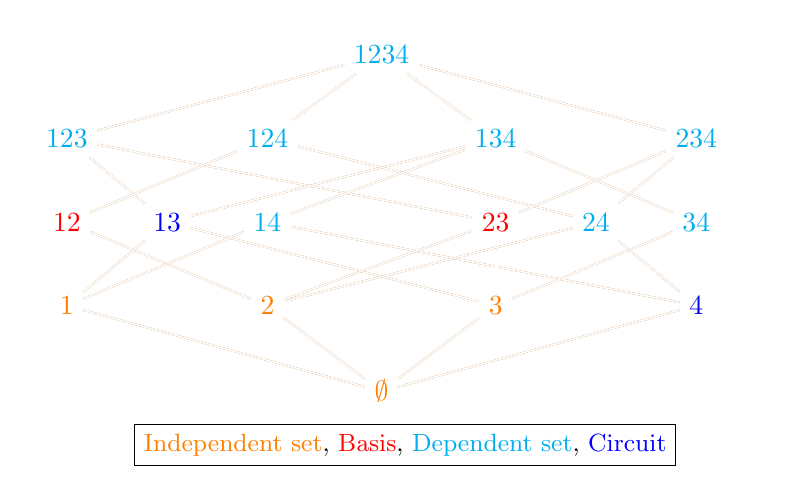
\begin{tikzpicture}
\matrix (a) [matrix of math nodes, column sep=0.6cm, row sep=0.6cm,]{
 & & &\textcolor{cyan}{
1234} & & & &\\
 \textcolor{cyan}{
123}& &\textcolor{cyan}{
124} & &\textcolor{cyan}{
134} &  & \textcolor{cyan}{
234}  \\
\textcolor{red}{12} & \textcolor{blue}{13} & \textcolor{cyan}{14} & & \textcolor{red}{23} & \textcolor{cyan}{
24} & \textcolor{cyan}{
34} \\
\textcolor{orange}{1}& &\textcolor{orange}{2} & & \textcolor{orange}{3}& & \textcolor{blue}{4} \\
& & & \textcolor{orange}{\emptyset} &  & & \\
&&&&&& \\};

\foreach \i/\j in {1-4/2-1, 1-4/2-3, 1-4/2-5, 1-4/2-7, 2-1/3-1, 2-1/3-2, 2-1/3-5, 2-3/3-1, 2-3/3-3, 2-3/3-6, 2-5/3-2, 2-5/3-3, 2-5/3-7, 2-7/3-5, 2-7/3-6, 2-7/3-7, 3-1/4-1, 3-1/4-3, 3-2/4-1, 3-2/4-5, 3-3/4-1, 3-3/4-7, 3-5/4-3, 3-5/4-5, 3-6/4-3, 3-6/4-7, 3-7/4-7, 3-7/4-5, 4-1/5-4, 4-3/5-4, 4-5/5-4, 4-7/5-4}
\draw[double, line width = 0.005mm, color = brown] (a-\i) -- (a-\j);

\node[draw] at (0, -2.5){\small \textcolor{orange}{Independent set}, \textcolor{red}{Basis}, \textcolor{cyan}{Dependent set}, \textcolor{blue}{Circuit}};
% \caption{Figure 3: Diagram of a 4-element matroid}
\end{tikzpicture}
\caption{Diagram of a 4-element matroid, with circuits in blue}
\label{fig:1234-matroid-circuits}
\end{center}
\end{figure}

\begin{exmp}
To get an intuition behind (C3), let us consider the matroid induced by the graph in figure (\ref{fig:amogus}). We will discuss graphic matroids later, but for now consider cycles of the graph as circuits. The diagram highlights two circuits --- $C_1$ and $C_2$ --- that share an edge ($e$). Taking the union of both circuits and removing $e$ yields a subgraph contains another cycle --- circuit $C_3$.
\end{exmp}


\begin{figure}[h]
\caption{A graph of suspicious shape, having three cycles.}
\label{fig:amogus}
\begin{subfigure}[h]{0.245\textwidth}
  \caption{Graph}
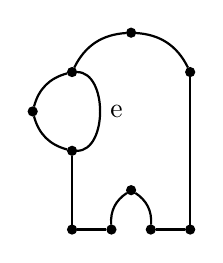
\begin{tikzpicture}[node distance={10mm}, thick, main/.style = {draw,circle,fill,inner sep=1pt}] 
  \node[main] (1) at (0,0) {}; 
  \node[main] (3) at (-0.5,0.5) {}; 
  \node[main] (4) at (0, 1) {}; 
  \node[main] (5) at (0, -1) {}; 
  \node[main] (6) at (1.5, -1) {}; 
  \node[main] (7) at (0.75, 1.5) {}; 
  \node[main] (8) at (1.5, 1) {}; 
  \node[main] (9) at (0.5, -1) {}; 
  \node[main] (10) at (1, -1) {}; 
  \node[main] (11) at (0.75, -0.5) {}; 
  \draw (1) to [bend left] (3);
  \draw (1) to [bend right=90]
node[midway, right] {e} (4) ;
  \draw (3) to [bend left] (4);
  \draw (4) to [bend left] (7);
  \draw (7) to [bend left] (8);
  \draw (8) to (6);
  \draw (5) to (9);
  \draw (6) to (10);
  \draw (9) to [bend left] (11);
  \draw (10) to [bend right] (11);
  \draw (5) to (1);
\end{tikzpicture} 
\end{subfigure}
\begin{subfigure}[h]{0.245\textwidth}
  \caption{$C _1$}
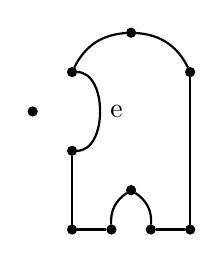
\begin{tikzpicture}[node distance={10mm}, thick, main/.style = {draw,circle,fill,inner sep=1pt}] 
  \node[main] (1) at (0,0) {}; 
  \node[main] (3) at (-0.5,0.5) {}; 
  \node[main] (4) at (0, 1) {}; 
  \node[main] (5) at (0, -1) {}; 
  \node[main] (6) at (1.5, -1) {}; 
  \node[main] (7) at (0.75, 1.5) {}; 
  \node[main] (8) at (1.5, 1) {}; 
  \node[main] (9) at (0.5, -1) {}; 
  \node[main] (10) at (1, -1) {}; 
  \node[main] (11) at (0.75, -0.5) {}; 
  \draw (1) to [bend right=90]
node[midway, right] {e} (4) ;
  \draw (4) to [bend left] (7);
  \draw (7) to [bend left] (8);
  \draw (8) to (6);
  \draw (5) to (9);
  \draw (6) to (10);
  \draw (9) to [bend left] (11);
  \draw (10) to [bend right] (11);
  \draw (5) to (1);
\end{tikzpicture} 
\end{subfigure}
\begin{subfigure}[h]{0.245\textwidth}
  \caption{$C _2$}
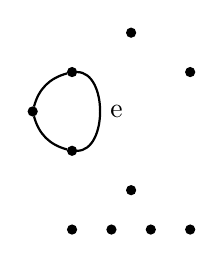
\begin{tikzpicture}[node distance={10mm}, thick, main/.style = {draw,circle,fill,inner sep=1pt}] 
  \node[main] (1) at (0,0) {}; 
  \node[main] (3) at (-0.5,0.5) {}; 
  \node[main] (4) at (0, 1) {}; 
  \node[main] (5) at (0, -1) {}; 
  \node[main] (6) at (1.5, -1) {}; 
  \node[main] (7) at (0.75, 1.5) {}; 
  \node[main] (8) at (1.5, 1) {}; 
  \node[main] (9) at (0.5, -1) {}; 
  \node[main] (10) at (1, -1) {}; 
  \node[main] (11) at (0.75, -0.5) {}; 
  \draw (1) to [bend left] (3);
  \draw (1) to [bend right=90]
node[midway, right] {e} (4) ;
  \draw (3) to [bend left] (4);
\end{tikzpicture} 
\end{subfigure}
\begin{subfigure}[h]{0.245\textwidth}
  \caption{$C _3$} 
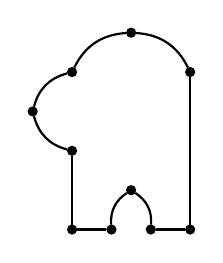
\begin{tikzpicture}[node distance={10mm}, thick, main/.style = {draw,circle,fill,inner sep=1pt}] 
  \node[main] (1) at (0,0) {}; 
  \node[main] (3) at (-0.5,0.5) {}; 
  \node[main] (4) at (0, 1) {}; 
  \node[main] (5) at (0, -1) {}; 
  \node[main] (6) at (1.5, -1) {}; 
  \node[main] (7) at (0.75, 1.5) {}; 
  \node[main] (8) at (1.5, 1) {}; 
  \node[main] (9) at (0.5, -1) {}; 
  \node[main] (10) at (1, -1) {}; 
  \node[main] (11) at (0.75, -0.5) {}; 
  \draw (1) to [bend left] (3);
  \draw (3) to [bend left] (4);
  \draw (4) to [bend left] (7);
  \draw (7) to [bend left] (8);
  \draw (8) to (6);
  \draw (5) to (9);
  \draw (6) to (10);
  \draw (9) to [bend left] (11);
  \draw (10) to [bend right] (11);
  \draw (5) to (1);
\end{tikzpicture} 
\end{subfigure}
                  \end{figure}

% We can say that a set $X \subseteq E$ is independent if and only if, it does not contain any circuit.
% The concept of circuits points towards something similar to a complement of the independent sets, but not completely. It is only the minimal dependent, and not all dependet subsets. We now have the following theorem.

\begin{lemma}\label{lem:circuits-have-properties}
  All circuits in a matroid satisfy (C1), (C2) and (C3).
\end{lemma}

\begin{proof} We will prove each property individually:
  
\begin{enumerate}
    \item[(C1)] $\emptyset \in \mathcal I$, therefore $\emptyset$ is not dependent (which means it cannot be a circuit)
    \item[(C2)] A counterexample to this clause would violate $C _2$ being minimal.
    \item[(C3)] Assume a counterexample exists. Because $C _1 \cup C _2 - e$ does not contain a circuit, it must be an element of $\mathcal I$. 

        We claim that $C _2 \setminus C _1$ is nonempty. Assume this is not the case. That would imply $C _2 \subseteq C _1$, but $C _1 \neq C _2 $ by (C3), which means that $C _1 $ is a proper subset of $C _2$. As both $C _1 $ and $C _2 $ are members of $\mathcal C$, this violates (C2), and is a contradiction. We can then assume some $f \in C _2 \setminus C _1 $ exists.

        As $C _2$ is minimally dependent, we know that $C _2 - f$ is independent. Let $I$ be a maximal independent subset of $C _2 \cup C _1$ which is a superset of $C _2 - f$. Clearly, $f \not\in I$ (otherwise $C _2 \subseteq I \in \mathcal I$). Furthermore, as $C _1 $ is a circuit, we know that $C _1 \not \subseteq I \in \mathcal I$ (otherwise $C _1$ would be independent). This means some $g \in C _1$ exists such that $g \not\in I$. As $f \in C _2  \setminus  C _2$, we know that $f \neq g$.

        As $I \subseteq C _1 \cup C _2$ and $f, g \in C _1 \cup C _2$ but $f, g \not\in I$, we can infer that 
        \begin{align*}
        |I| \leq |C _1 \cup C _2 - f - g| = |C _1 \cup C _2| - 2.
        \end{align*}

        We also notice that $|C _1 \cup C _2 - e| = |C _1 \cup C _2 | - 1$. We can now conclude by transitivity with $|C _1 \cup C _2 | - 2 < |C _1 \cup C _2 | - 1$ that $|I| < |C _1 \cup C _2 - e|$. We recall that both $I$ and $C _1 \cup C _2 - e$ are members of $\mathcal I$. We can apply (I3) to generate a superset of $I$ which contradicts it's maximality.
\end{enumerate}
\end{proof}

\begin{theorem}\label{thm:matroid-circuit-definition}
Let $E$ be a set and $\mathcal C$ be a collection of subsets of $E$ which satisfies the conditions outlined above. Let  $\mathcal I$  be the collection of subsets of $E$ that contain no member of $\mathcal C$, that is 

\begin{align}
   % \forall X \in \mathcal{I}, \forall C \in \mathcal C,  C \not \subseteq X. 
   \mathcal{I} = \{I \in 2^E |\; \text{for all } \; C \in \mathcal{C}\; \text{we have} \; C \not\subseteq I\}
    \label{independent-sets-from-circuits}
\end{align}

    The pair $(E,\mathcal I)$ is a matroid having $\mathcal C$ as its collection of circuits.
\end{theorem}

\begin{proof} We start by showing that $\mathcal I $ satisfies the necessary conditions for $(E, \mathcal I )$ to be a matroid:
    \begin{enumerate} 
        \item[(I1)] The only subset of $\emptyset $ is $ \emptyset $, but $ \emptyset \not\in \mathcal C $, so $ \emptyset $ satisfies (\ref{independent-sets-from-circuits}), hence $\emptyset \in \mathcal I$.
        \item[(I2)] Assume we have $X \subseteq Y \in \mathcal I$. Assume that $X \not\in I$, i.e.\ there exists some $C \in \mathcal C $ such that $C \subseteq X$. We recall that $\subseteq $ is transitive, thus $C \subseteq Y$ and $Y \not\in I$, hence a contradiction.
        \item[(I3)] Given $X, Y \in \mathcal I $ with $|X| < |Y|$ we must show there exists some $e \in Y \setminus X$ such that $X \cup \{e\} \in \mathcal I$. Assume that such an $e$ does not exist, i.e.\ for all $e \in Y \setminus X$ we have some circuit $C _e \in \mathcal C $ such that $C _e \subseteq X \cup \{e\}$. We obviously have $e \in C_e$, because otherwise $C_e \subseteq X$ and $X \not\in \mathcal I$.


     Let $X' = X \setminus Y$ and $Y' = Y \setminus X$. We will prove the statement by induction: given some set $S \subseteq X'$, a set of circuits $D \subseteq \mathcal C$ with $\forall C \in D, C \subseteq  S \cup Y$ and a surjective but not injective function $f : D \to S$ such that $f(D)$ is maximal in size and $\forall C \in D, f(C) \in C$, our statement is proven. We will use induction on the size of $S$:
    \begin{enumerate}
      \item If $S = \{e\}$ only has one element, we know that $f$ is not injective, so we must have distinct $C _1, C _2 \in D$ such that $e = f(C _1 ) = f(C _2)$. We can use the $3$-rd circuit axiom to generate some circuit $C _3 \subseteq C _1 \cup C _2 - e$. We recall that $C _1 , C _2 \subseteq S \cup Y $, so $C _3 \subseteq S \cup Y - e$ which implies $C _3 \subseteq Y$, which is a contradiction.
        \item Inductive step. Assuming the statement is true for all choices of $S$ with $k$ elements, we will attempt to prove it is also true when $S$ has $k + 1$ elements. Recalling that $f$ is not injective, we must have distinct $C _1, C _2 \in D$ such that $f(C _1 ) = f(C _2)$. Let $g = f(C _1)$. We have $g \in C _1, C _2$, so by the $3$-rd circuit axiom we must have some circuit $C  _3 \subseteq C _1 \cup C _2 - g$. Let $S' = C _3 \cap X'$. 

            For all $e \in S'$, we claim there must exist some $C_e \in D$ such that $e = f(C_e)$. Assume this is not the case, i.e.\ there is some $e \in S'$ such that no valid choice of $C_e$ exists. Given that $e \in S'$, we know that either $e \in C_1$ or $e \in C_2$. After a potential swap, we assume that $e \in C_1$. We can now define $f'(C) = e$ when $C = C_1$ and $f'(C) = f(C)$. Because no choice of $C_e$ exists, we know that $e \not\in f(D)$. Because $f(C _1 ) = f(C _2 )$ we have $f(D) = f(D - C _1 )$ which lets us compute $f'(D) = f(D) \cup \{e\}$, which means $f(D)$ was not maximal, hence a contradiction. Our claim is then true.

            Define $D' = \{C_e | e \in S'\} \cup \{C _3 \}$. We've essentially proven in the last paragraph that $f : \{C_e | e \in S'\} \to S'$ is still a  surjective function. It then follows that $h = f : D' \to S'$ is surjective as well. By the Pigeonhole principle, we know $h$ cannot be injective, because $|D'| = |S'| + 1$. We are now almost ready to apply the induction hypothesis to $(S', D', h)$. We've shown a choice for $h$ exist. If this choice is not maximal, swap it with a maximal choice (we had to show that at least one choice exists for a maximal choice to exist). We can now apply the induction hypothesis, proving the statement.
    \end{enumerate}

    We notice that $X$ can be partitioned into $X'$ and $X \cap Y$, hence $|X| = |X'| + |X \cap Y|$. We can follow a similar process for $Y$. Combining the two together with the fact that $|X| < |Y|$ yields that $|X'| < |Y'|$. We know that $Y \in \mathcal I$ so $\forall e \in Y', C_e \not \subseteq  Y$, but $C_e \subseteq  X \cup \{e\}$ therefore there must exist some $c_e \in C_e \cap X'$. 

    We define $D = \{C_e, e \in Y'\}$, $f(C_e) = c_e$ and $S = f(D)$. Furthermore, we know that $f$ is not injective by the Pigeonhole principle (we have $|D| = |Y'| > |X'| \geq |S|$). We also know, by the definition of $S$, that $f$ is surjective. We've shown a choice of $f$ exists. If it is not maximal, swap it with a maximal choice. We can now apply the statement proven by induction to finish the proof.
\end{enumerate}


We now show that $C$ is a circuit for the newly defined matroid if and only if it is a member of $\mathcal C$. 
\begin{enumerate}
  \item[$\implies$]
  If $C$ is a circuit, then $C \not\in \mathcal I$, which means that $C$ contains some $D \in \mathcal C$. As $C$ is minimally dependent, all its proper subsets are independent, but members of $\mathcal C$ cannot be independent (as seen in the definition of $\mathcal I$), which implies that $C = D$, hence $C \in \mathcal C$.
  \item[$\impliedby$]
  Let $C \in \mathcal C$. Assume $C$ is not a circuit. Clearly, $C \not\in \mathcal I$ is implied by the definition of $\mathcal I$ seen above. This implies that $C$ is dependent but not a circuit, which means $C$ is not miminal. 

  A proper subset $D  \subseteqneq C$ must then exist such that $D$ is a circuit. We've already shown in the $\implies$ direction how this implies $D \in \mathcal C$. We have now constructed a contradiction to (C2), hence our assumption that such a circuit exists is false.

\end{enumerate}



  We can now conclude that $(E, \mathcal I)$ is indeed a matroid with $\mathcal C$ as it's set of circuits.
\end{proof}

\section{Graphic matroids}

TRYING TO DO GRAPHS, DONT LAUGH!!

\tikz \graph {A -> {b,c} -> }



\section{Rank Function}

The rank function is a function $r:2^E \rightarrow \mathbb{Z}_{\geq0}$ that, when given a $X\subseteq E(M)$, gives you the cardinality of the maximal independent set contained in $X$. In other words:
$$ r(X) = \max\{\, |I| : I\in\mathcal{I} \text{ and } I\subseteq X \} $$
For example, $r(M):=r(E(M))=|B|$ for some $B\in\mathcal{B}(M)$. Like all the previous times, we can characterize the rank function with the following properties:

\begin{defn}
    Let $E$ be a non-empty finite set, and let $\rank : 2^E \rightarrow \mathbb{Z}_{\geq0}$ be a function satisfying:
    \begin{enumerate}
        \item[(R1)] If $X\subseteq E$, then $0 \leq \rank(X) \leq |X| $
        \item[(R2)] If $X\subseteq Y\subseteq E$, then $\rank(X)\leq\rank(Y)$
        \item[(R3)] If $X,Y\subseteq E$, then $\rank(X\cup Y)+\rank(X\cap Y) \leq \rank(X)+\rank(Y) $
    \end{enumerate}
\end{defn}

Below, we again find our example matroid drawing. This time, instead of using a new color, we will denote the rank of each set by writing it in subscript below the set. We can see that the rank of any set is at most its cardinality, and each subset of some set has at most the rank of that set. As always, it takes a bit more effort to show that the last property holds for a given matroid.

\begin{center}
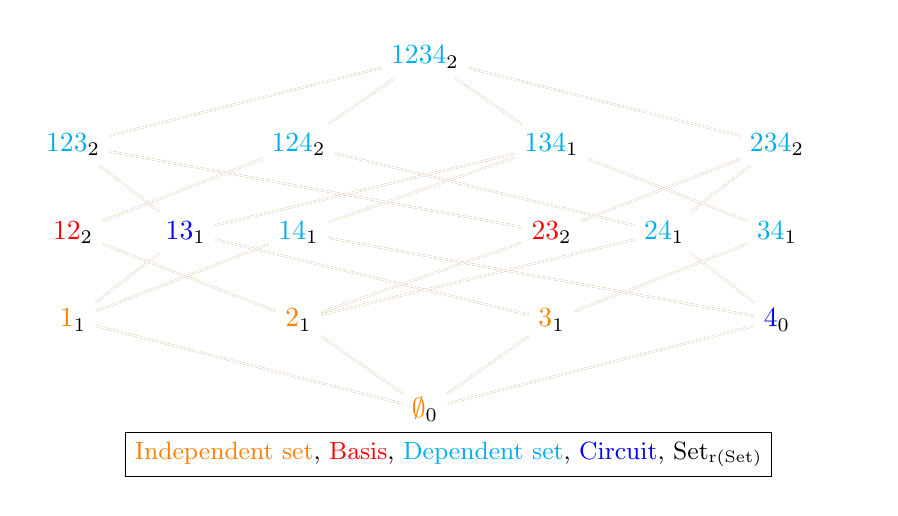
\begin{tikzpicture}

\matrix (a) [matrix of math nodes, column sep=0.6cm, row sep=0.6cm,]{
 & & &\textcolor{cyan}{
1234}_2 & & & &\\
 \textcolor{cyan}{
123}_2& &\textcolor{cyan}{
124}_2 & &\textcolor{cyan}{
134}_1 &  & \textcolor{cyan}{
234}_2  \\
\textcolor{red}{12}_2 & \textcolor{blue}{13}_1 & \textcolor{cyan}{14}_1 & & \textcolor{red}{23}_2 & \textcolor{cyan}{
24}_1 & \textcolor{cyan}{
34}_1 \\
\textcolor{orange}{1}_1& &\textcolor{orange}{2}_1 & & \textcolor{orange}{3}_1& & \textcolor{blue}{4}_0 \\
& & & \textcolor{orange}{\emptyset}_0 &  & & \\
&&&&&& \\};

\foreach \i/\j in {1-4/2-1, 1-4/2-3, 1-4/2-5, 1-4/2-7, 2-1/3-1, 2-1/3-2, 2-1/3-5, 2-3/3-1, 2-3/3-3, 2-3/3-6, 2-5/3-2, 2-5/3-3, 2-5/3-7, 2-7/3-5, 2-7/3-6, 2-7/3-7, 3-1/4-1, 3-1/4-3, 3-2/4-1, 3-2/4-5, 3-3/4-1, 3-3/4-7, 3-5/4-3, 3-5/4-5, 3-6/4-3, 3-6/4-7, 3-7/4-7, 3-7/4-5, 4-1/5-4, 4-3/5-4, 4-5/5-4, 4-7/5-4}
\draw[double, line width = 0.005mm, color = brown] (a-\i) -- (a-\j);

\node[draw] at (0, -2.5){\small \textcolor{orange}{Independent set}, \textcolor{red}{Basis}, \textcolor{cyan}{Dependent set}, \textcolor{blue}{Circuit}, $\text{Set}_{\rank(\text{Set})}$ };

\end{tikzpicture}
\end{center}

Now, let us prove that the rank function of a matroid satisfy these properties:

\begin{proof}
    \,
    \begin{enumerate}
        \item Since the co-domain is $\mathbb{Z}_{\geq0}$, $0\leq\rank(X)$. Since the maximal independent set contained in $X$ is... contained in $X$, the cardinality of that set must be smaller or equal to $|X|$. Thus, $0\leq\rank(X)\leq|X|$.
        \item Let $I_X$ be a minimal independent set contained in $X$, so $\rank(X)=|I_X|$. $I_X\subseteq X\subseteq Y$ implies that $I_X$ is an independent set contained in $Y$. Since $I_X$ may or may not be a maximal independent set contained in $Y$, $\rank(X)=|I_X|\leq\rank(Y)$. 
        \item We assume that $A\subseteq B\subseteq E$. Let $I_{A\cap B}$ be a maximal independent set contained in $A\cap B$. Since $A\cap B\subseteq A\cup B$, $I_{A\cap B}$ must be an independent set contained in $A\cup B$. Let $I_{A\cup B}$ be $I_{A\cap B}$ extended to be a \textbf{maximal} independent set contained in $A\cup B$. 
        
        Now, et us take a look at $I_{A\cup B}\cap A$. Since the set is contained in $A$, (I2) tells us that $I_{A\cup B}\cap A$ is in independent set contained in $A$. Since the set may or may not be maximal in that regard, $|I_{A\cup B}\cap A|\leq \rank(A)$. Similarly, $|I_{A\cup B}\cap B|\leq \rank(B) $.
        
        $$ \rank(X)+\rank(Y) \geq |I_{A\cup B}\cap A|+|I_{A\cup B}\cap B| $$
        $$ = |(I_{A\cup B}\cap A)\cup(I_{A\cup B}\cap B)|+|(I_{A\cup B}\cap A)\cap(I_{A\cup B}\cap B)| $$
        $$ = |I_{A\cup B}\cap (A\cup B)|+|I_{A\cup B}\cap (A\cap B)| $$

        Since $I_{A\cup B}\subseteq A\cup B$, $I_{A\cup B}\cap(A\cup B) = I_{A\cup B}$.

        Since $I_{A\cap B}\subseteq I_{A\cup B}$, $I_{A\cup B}\cap (A\cap B) \supset I_{A\cap B}\cap (A\cap B) = I_{A\cap B} $. Let $e\in I_{A\cup B}\cap (A\cap B)$. Aiming for contradiction, suppose $e\notin I_{A\cap B}$. Since $I_{A\cap B}\cup e \subseteq I_{A\cup B} $, $I_{A\cap B}\cup e$ must be an independent set contained in $A\cap B$. This contradicts the fact that $I_{A\cap B}$ is a maximal in that regard. Thus, $e\in I_{A\cap B}$. This proves that $I_{A\cup B}\cap(A\cap B)\subseteq I_{A\cap B} $, which implies equality between the two sets.

        Thus,

        $$ \rank(X)+\rank(Y) \geq |I_{A\cup B}|+|I_{A\cap B}| = \rank(A\cup B)+\rank(A\cap B) $$
    \end{enumerate}
\end{proof}
One might observe that the rank of an independent set is the cardinality of the set itself. This is because the largest independent set that is contained in this independent set is of course the independent set itself. With this property, we can define the set of independent sets with the three properties of the rank function.
\begin{theorem}
    Let $E$ be a finite set, and let $\rank : 2^E \rightarrow \mathbb{Z}_{\geq0}$ be a function satisfying (R1)-(R3). Let $\mathcal{I} = \{ I\subseteq E : \rank(I)=|I| \} $. Then $(E,\mathcal{I})$ is a matroid with $\rank$ as its rank function.
\end{theorem}
Before we prove this, let's prove this small theorem first:
\begin{theorem}
\label{rankextension}
    Let $E$ be a finite set and $\rank:2^E\rightarrow \mathbb{Z}_{\geq0}$ be a function satisfying (R2) and (R3). Let $X,Y\subseteq E$. Then if for all $y\in Y-X$, $\rank(X\cup y)=\rank(X)$, then $\rank(X\cup Y)=\rank(Y)$.
\end{theorem}
\begin{proof}
    We will prove that the statement holds with $Y-X = \{a_1,a_2,\dots,a_k\}$ holds for all integers $k$.
    \begin{enumerate}
        \item Base case: $k=1$

        If $\rank(X\cup a_1)=\rank(X)$, then $\rank(X\cup Y)=\rank(X\cup(Y-X))=\rank(X\cup a_1)=\rank(X)$.
        \item Induction Step: Assume the statement holds for $k=n$.
        \item Let $k=n+1$: Assume that $Y-X=\{a_1,\dots,a_{n+1}\}$ for all $i\in\{1,\dots,n+1\}$ $\rank(X\cup a_i)=\rank(X)$. Then, using the assumption and our induction assumption, 
        $$ \rank(X)+\rank(X) = \rank(X\cup \{a_1,\dots,a_n\})+\rank(X\cup a_{n+1}) $$
        Using (R3), we get
        $$ \geq \rank([X\cup\{a_1,\dots,a_n\}]\cup [X\cup a_{n+1}]) + \rank([X\cup\{a_1,\dots,a_n\}]\cap [X\cup a_{n+1}]) $$
        $$ = \rank(X\cup\{a_1,\dots,a_{n+1}\}) + \rank(X) $$
        Using (R2), we get
        $$ \geq \rank(X)+\rank(X) $$
        Since $\rank(X)+\rank(X)$ is on both sides, equality holds throughout. Thus, $\rank(X\cup\{a_1,\dots,a_{n+1}\})=\rank(X\cup Y)=\rank(X)$. And thus, the statement holds for $k=n+1$.
    \end{enumerate}
    Thus, by mathematical induction, the statement holds for all integers $k$.
\end{proof}
Finally, we can prove Theorem 5:
\begin{proof}
    To prove that $(E,\mathcal{I})$ is a matroid, we will check if $\mathcal{I}$ satisfies (I1)-(I3).
    \begin{enumerate}
        \item (R1) tells us that $0\leq\rank(\emptyset)\leq|\emptyset|=0$, which implies that $\rank(\emptyset)=0=|\emptyset|$, which means that $\emptyset\in\mathcal{I}$, so (I1) is satisfied.
        \item Assume we have $J\subseteq I\in\mathcal{I}$. Then, using (R3),
        $$ \rank(J)+\rank(I-J) \geq \rank(J\cup[I-J])+\rank(J\cap[I-J]) = \rank(I)+\rank(\emptyset)=|I| $$
        Using (R2), we also get that
        $$ \rank(J)+\rank(I-J) \leq |J|+\rank(I-J) \leq |J|+|I-J| = |I| $$
        This implies that equality must hold throughout. At last, we show that
        $$ \rank(J)+\rank(I-J) = |J|+\rank(I-J) \Rightarrow \rank(J)=|J| $$
        Thus, $J\in\mathcal{I}$, so {I2} is satisfied.
        
        \item Suppose (I3) does not hold for some $I,J\in\mathcal{I}$ with $|I|>|J|$. Then for all $e\in I-J$, $J\cup e\notin \mathcal{I}$. Also, remember that $I,J\in\mathcal{I}$ means that $\rank(I)=|I|$ and $\rank(J)=|J|$.

        Since $J\subseteq J\cup e$, we can use (R1) and (R2) to see that
        $$ |J|=\rank(J)\leq\rank(J\cup e)|\leq|J\cup e|=|J|+1 $$
        $J\cup e\notin \mathcal{I}$ tells us that $\rank(J\cup e)\neq|J\cup e|$, so that must mean that $\rank(J\cup e)$ is equal to what's on the left-hand side, so $\rank(J)$.

        This gives us that for all $e\in I-J$, $\rank(J\cup e)=\rank(J)$, which, according to Theorem 6, implies that $\rank(J\cup I)=\rank(J)=|J|$. However, since $I\subseteq J\cup I$, (R2) tells us that $\rank(J\cup I) \geq \rank(I) = |I|$, which means that $|J|\geq|I|$. This contradicts our assumption that $|J|<|I|$. Thus, (I3) is satisfied.
    \end{enumerate}
    Thus, $(E,\mathcal{I})$ is a matroid.
\end{proof}


\section{Graphic matroids}

TRYING TO DO GRAPHS, DONT LAUGH!!

\tikz \graph {A -> {b,c} -> }



\newpage
\section{Rank Function}

We will introduce our first description of matroids that does not rely on a collection of subsets that satisfies certain properties, but rather on a \textit{function} that satisfies certain properties.

The rank function is a function $\rank :2^E \rightarrow \mathbb{Z}_{\geq0}$ that, given a $X\subseteq E(M)$, gives you the cardinality of a maximal independent set contained in $X$. In other words:

$$ \rank(X) = \max\{\, |I| \; | \,\, I\in\mathcal{I} \text{ and } I\subseteq X \}. $$
For example, $\rank(E(M))=|B|$ for some $B\in\mathcal{B}(M)$, and we define $\rank(M) = \rank(E(M))$. We can characterize the rank function with the following properties:

\begin{theorem}
    Let $M$ be a matroid on a ground set $E$, and let $\rank : 2^E \rightarrow \mathbb{Z}_{\geq0}$ be its rank function. Then $\rank$ satisfies these properties.
    \begin{enumerate}
        \item[(R1)] If $X\subseteq E$, then $0 \leq \rank(X) \leq |X| $
        \item[(R2)] If $X\subseteq Y\subseteq E$, then $\rank(X)\leq\rank(Y)$
        \item[(R3)] If $X,Y\subseteq E$, then $\rank(X\cup Y)+\rank(X\cap Y) \leq \rank(X)+\rank(Y) $
    \end{enumerate}
\end{theorem}

In figure (\ref{fig:1234-matroid-rank}) we again find our example matroid drawing. We denote the rank of each set by writing it in subscript below the set. We can see that the rank of any set is at most its cardinality, and each subset of some set has at most the rank of that set. As always, it takes a bit more effort to show that the last property holds for a given matroid.

\begin{figure}[H]
    \begin{center}
    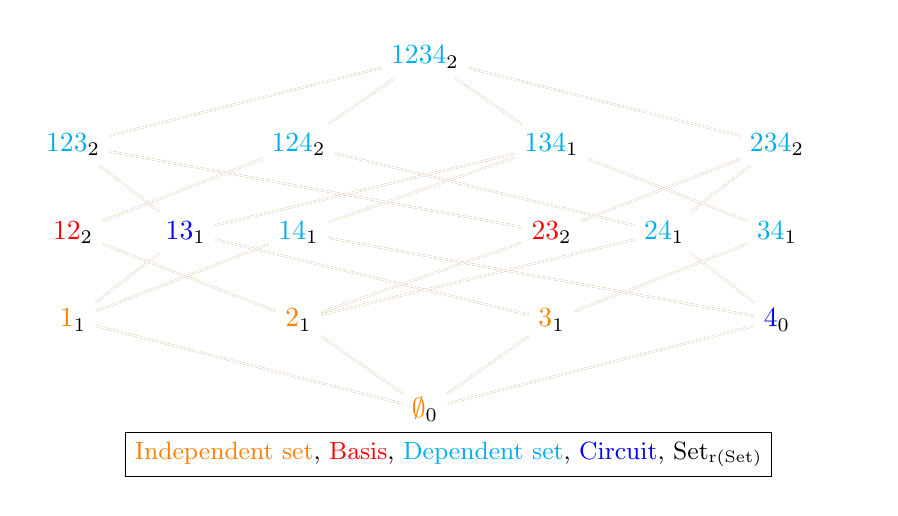
\begin{tikzpicture}
    
    \matrix (a) [matrix of math nodes, column sep=0.6cm, row sep=0.6cm,]{
     & & &\textcolor{cyan}{
    1234}_2 & & & &\\
     \textcolor{cyan}{
    123}_2& &\textcolor{cyan}{
    124}_2 & &\textcolor{cyan}{
    134}_1 &  & \textcolor{cyan}{
    234}_2  \\
    \textcolor{red}{12}_2 & \textcolor{blue}{13}_1 & \textcolor{cyan}{14}_1 & & \textcolor{red}{23}_2 & \textcolor{cyan}{
    24}_1 & \textcolor{cyan}{
    34}_1 \\
    \textcolor{orange}{1}_1& &\textcolor{orange}{2}_1 & & \textcolor{orange}{3}_1& & \textcolor{blue}{4}_0 \\
    & & & \textcolor{orange}{\emptyset}_0 &  & & \\
    &&&&&& \\};
    
    \foreach \i/\j in {1-4/2-1, 1-4/2-3, 1-4/2-5, 1-4/2-7, 2-1/3-1, 2-1/3-2, 2-1/3-5, 2-3/3-1, 2-3/3-3, 2-3/3-6, 2-5/3-2, 2-5/3-3, 2-5/3-7, 2-7/3-5, 2-7/3-6, 2-7/3-7, 3-1/4-1, 3-1/4-3, 3-2/4-1, 3-2/4-5, 3-3/4-1, 3-3/4-7, 3-5/4-3, 3-5/4-5, 3-6/4-3, 3-6/4-7, 3-7/4-7, 3-7/4-5, 4-1/5-4, 4-3/5-4, 4-5/5-4, 4-7/5-4}
    \draw[double, line width = 0.005mm, color = brown] (a-\i) -- (a-\j);
    
    \node[draw] at (0, -2.5){\small \textcolor{orange}{Independent set}, \textcolor{red}{Basis}, \textcolor{cyan}{Dependent set}, \textcolor{blue}{Circuit}, $\text{Set}_{\rank(\text{Set})}$ };
    \end{tikzpicture}
    \end{center}

    \caption{Description of a 4-element matroid, with the rank of each set as subscript.}
    \label{fig:1234-matroid-rank}
\end{figure}




Now, let us prove that the rank function of a matroid satisfies these properties. 

\begin{proof}
    \begin{enumerate} This proof was inspired by \cite[p. 23]{oxley1}.
        \item[(R1)] Since the co-domain of $\rank$ is $\mathbb{Z}_{\geq0}$ then  $\rank(X) \geq 0$. Let $I_X$ be a maximal independent set contained in $X$. By definition, we see that $|I_X|=\rank(X)$. Since $X\supseteq I_X$, it follows that $|X| \geq |I_X| = \rank(X)$.       Thus, $0\leq\rank(X)\leq|X|$ what we wanted to show.
        
        \item[(R2)] Let $I_X$ be a minimal independent set contained in $X$, so $\rank(X)=|I_X|$. $I_X\subseteq X\subseteq Y$ implies that $I_X$ is an independent set contained in $Y$. Since $I_X$ is an independent set contained in $Y$ then by definition $|I_X|\leq \rank(Y)$ since $\rank(Y)$ is the size of the \textit{largest} independent set contained in $Y$. Finally, we get that $\rank(X)=|I_X|\leq \rank(Y)$ what we wanted to show.
        
        \item[(R3)] We assume that $A\subseteq B\subseteq E$. Let $I_{A\cap B}$ be a maximal independent set contained in $A\cap B$. Since $A\cap B\subseteq A\cup B$, it means that $I_{A\cap B}$ must be an independent set contained in $A\cup B$. Let $I_{A\cup B}$ be $I_{A\cap B}$ \textit{extended} to be a \textbf{maximal} independent set contained in $A\cup B$. So $I_{A\cap B}\subseteq I_{A\cup B} \subseteq A\cup B$. 
        
        Now, let us take a look at the set $I_{A\cup B}\cap A$. Since the set is contained in $A$ and $I_{A\cup B}$, the property (I2) tells us that $I_{A\cup B}\cap A$ is in independent set contained in $A$. Since the set may or may not be maximal we know by definition, $|I_{A\cup B}\cap A|\leq \rank(A)$. Similarly, $|I_{A\cup B}\cap B|\leq \rank(B) $.

        We will now use the well known fact that for any sets $X$ and $Y$, it holds that $|X\cup Y|=|X|+|Y|-|X\cap Y|$, in other words $|X|+|Y|=|X\cup Y|+|X\cap Y|$.
        
        \begin{align*}
            \rank(A)+\rank(B) &\geq |I_{A\cup B}\cap A|+|I_{A\cup B}\cap B| 
            \\&=  |(I_{A\cup B}\cap A)\cup(I_{A\cup B}\cap B)|
             +|(I_{A\cup B}\cap A)\cap(I_{A\cup B}\cap B)| 
            \\&=  |I_{A\cup B}\cap (A\cup B)|+|I_{A\cup B}\cap (A\cap B)|. 
        \end{align*}

        Since $I_{A\cup B}\subseteq A\cup B$, we see that $I_{A\cup B}\cap(A\cup B) = I_{A\cup B}$.

        Because $I_{A\cap B}\subseteq I_{A\cup B}$ and $I_{A\cap B}\subseteq A\cap B$, it tells us that $I_{A\cup B}\cap (A\cap B) \supseteq I_{A\cap B}\cap (A\cap B) = I_{A\cap B} $. Let $e\in I_{A\cup B}\cap (A\cap B)$. Aiming for contradiction, suppose $e\notin I_{A\cap B}$. Since $e\in I_{A\cup B}$, we can see that $I_{A\cap B}\cup e \subseteq I_{A\cup B} $. Then (I2) implies that $I_{A\cap B}\cup e$ is independent. Combining that fact with that $e\in A\cap B$, we see that $I_{A\cap B}\cap e$ is an independent set contained in $A\cap B$. This contradicts the maximality of $I_{A\cap B}$ in being independent and contained in $A\cap B$. Thus, the contradiction gives us that $e\in I_{A\cap B}$. This proves that $I_{A\cup B}\cap(A\cap B)\subseteq I_{A\cap B} $, which implies equality between the two sets.

        Thus,

        $$ \rank(X)+\rank(Y) \geq  |I_{A\cup B}|+|I_{A\cap B}| = \rank(A\cup B)+\rank(A\cap B). $$
    \end{enumerate}
\end{proof}
One might observe that the rank of an independent set is the cardinality of the set itself. This is because the largest independent set that is contained in this independent set is of course the independent set itself. With this property, we can define the set of independent sets with the three properties of the rank function.
\begin{theorem}
    \label{thm:indep-from-bases}
    Let $E$ be a finite set, and let $\rank : 2^E \rightarrow \mathbb{Z}_{\geq0}$ be a function satisfying (R1)-(R3). Let $\mathcal{I} = \{ I\subseteq E : \rank(I)=|I| \} $. Then $(E,\mathcal{I})$ is a matroid with $\rank$ as its rank function.
\end{theorem}
Before we prove this, let us prove the following minor theorem first.
\begin{theorem}
\label{rankextension}
    Let $E$ be a finite set and $\rank:2^E\rightarrow \mathbb{Z}_{\geq0}$ be a function satisfying (R2) and (R3). Let $X,Y\subseteq E$. If for all $y\in Y-X$, it holds that $\rank(X\cup y)=\rank(X)$, then we have that $\rank(X\cup Y)=\rank(Y)$.
\end{theorem}
\begin{proof} 
    This proof was inspired by \cite[p. 24]{oxley1}. We will prove that the statement holds with $Y-X = \{a_1,a_2,\cdots,a_k\}$ for all integers $k$.
    \begin{enumerate}
        \item Consider the case when $k=1$. If $\rank(X\cup a_1)=\rank(X)$, then $\rank(X\cup Y)=\rank(X\cup(Y-X))=\rank(X\cup a_1)=\rank(X)$.
        \item Assume the statement holds for $k=n$. We will attempt to prove it also holds for $k = n + 1$.
        
        Let us see if the statement holds for $k=n+1$: Let $Y-X=\{a_1,\cdots,a_{n+1}\}$ and assume that for all $i\in\{1,\cdots,n+1\}$, it holds that $\rank(X\cup a_i)=\rank(X)$. Then, using the assumption and our induction hypothesis, 
        \begin{align*}
            \rank(X)+\rank(X) &= \rank(X\cup \{a_1,\cdots,a_n\})+\rank(X\cup a_{n+1}) 
            \\&\geq \rank\left(\left[X\cup\{a_1,\cdots,a_n\}\right]\cup \left[X\cup a_{n+1}\right]\right) +
             \\ &\quad\:  \rank\left([X\cup\{a_1,\cdots,a_n\}]\cap [X\cup a_{n+1}]\right)  && \text{(using (R3))}
            \\&= \rank\left(X\cup\{a_1,\cdots,a_{n+1}\}\right) + \rank\left(X\right) 
            \\&\geq \rank(X)+\rank(X).  && \text{(using (R2)) }
        \end{align*}
        Since $\rank(X)+\rank(X)$ is on both sides, equality holds throughout. 
        
        Thus, $\rank(X\cup Y) = \rank(X\cup\{a_1,\cdots,a_{n+1}\})=\rank(X)$. And thus, the statement holds for $k=n+1$.
    \end{enumerate}
    Thus, by mathematical induction, the statement holds for all integers $k$.
\end{proof}
Finally, we can prove Theorem 9:
\begin{proof}[Proof of theorem (\ref{thm:indep-from-bases})]
This proof was inspired by \cite[p. 24]{oxley1}. To prove that $(E,\mathcal{I})$ is a matroid, we will prove that $\mathcal{I}$ satisfies (I1)-(I3).
    \begin{enumerate}
        \item (R1) tells us that $0\leq\rank(\emptyset)\leq|\emptyset|=0$, which implies that $\rank(\emptyset)=0=|\emptyset|$. By how we defined $\mathcal{I}$, this implies that $\emptyset\in\mathcal{I}$, so (I1) is satisfied.
        \item Assume we have $J\subseteq I\in\mathcal{I}$. Then, using (R3),
        $$ \rank(J)+\rank(I-J) \geq \rank(J\cup[I-J])+\rank(J\cap[I-J]) = \rank(I)+\rank(\emptyset)=|I|. $$
        Using (R2), we also get that
        $$ \rank(J)+\rank(I-J) \leq |J|+\rank(I-J) \leq |J|+|I-J| = |I|. $$
        This implies that equality must hold throughout. At last, we show that
        $$ \rank(J)+\rank(I-J) = |J|+\rank(I-J) \Rightarrow \rank(J)=|J|. $$
        Since $\rank(J)=|J|$ means that $J\in\mathcal{I}$, we conclude that (I2) is satisfied.
        
        \item Suppose (I3) does not hold for some $I,J\in\mathcal{I}$ with $|I|>|J|$. Then for all $e\in I-J$, it holds that $J\cup e\notin \mathcal{I}$. Also, remember that $I,J\in\mathcal{I}$ means that $\rank(I)=|I|$ and $\rank(J)=|J|$.

        For this next part, let $e$ be anarbitrary member of $I-J$. Since $J\subseteq J\cup e$, we can use (R1) and (R2) to see that
        $$ |J|=\rank(J)\leq\rank(J\cup e)\leq|J\cup e|=|J|+1 .$$
        
       We see that $J\cup e\notin \mathcal{I}$ tells us that $\rank(J\cup e)\neq|J\cup e|=|J|+1$. Since we just proven that $|J|\leq\rank(J\cup e)\leq|J|+1$, it must mean that $\rank(J\cup e)$ is equal to what's on the left-hand side, so $|J|=\rank(J)$.

        This gives us that for all $e\in I-J$, it holds that $\rank(J\cup e)=\rank(J)$. With this, theorem (\ref{rankextension}) tells us that $\rank(J\cup I)=\rank(J)=|J|$. However, since $I\subseteq J\cup I$, we can use (R2) to see that $\rank(J\cup I) \geq \rank(I) = |I|$. Combining those two, we get that $|J|\geq|I|$. This contradicts our assumption that $|J|<|I|$. Thus, (I3) is satisfied.
    \end{enumerate}
    Thus, $(E,\mathcal{I})$ is a matroid.
\end{proof}




\section{Closure}


We will introduce one more important notion, the one of closure operator. As the name operator suggests, it is a map between objects of the same type. Our objects are of course the subsets of the ground set of a matroid. The idea of the closure operator is that it adds to any subset $X \subset E$ whatever is left in $E$ that does not change the rank when added to $X$. In doing so it will produce \textit{closed sets} which are in matroid theory called flats, another collection of subsets with distinctive properties. 

Closure will also admit desirable interpretation in the case of the prototypical examples of representable and graphic matroids. In the case of representable matroids, in will add to $X$ all elements which are in the vector span of $X$ and contained in $E$ (thus it will not increase the vector rank of $E$). In the case of graphic matroids it will add to any set of edges all edges that create cycles between its sets of vertices (thus will not increase the size of spanning forrest).

\begin{defn}
    Let $M = (E, \mathcal{I})$ be a matroid. The closure operator is a function $\cl: 2^E \to 2^E$ such that

    $$\cl(X) = \{x \in E\; | \; \rank(X \cup x) = \rank(X) \}.$$

    
\end{defn}

The operator has numerour important properties and we will immediatly also prove the reverse statement. Namely that these characteristic properties \textit{uniquely characterize} the closure operator of a matroid.

\begin{theorem}
Let $M = (E, \mathcal{I})$ be a matroid and $\cl: 2^E \to 2^E$ be a function. Then $\cl$ is the closure operator of $M$ \textbf{if and only if}

\begin{enumerate}
    \item For any $X \subset E$ we have $X \subset \cl (X)$
    \item If $X \subset Y \subset E$ then $\cl(X) \subset \cl(Y)$.
    \item For all $X$ we have $\cl(\cl(X)) = \cl(X)$

    \item Let $X \subset E$ and $b \in 
    \cl(X \cup a) - \cl(X)$ then $a \in \cl(X \cup b)$
\end{enumerate}
\end{theorem}


\begin{proof}
    All of the four statements in the only if direction (assuming $\cl$ is the closure operator) are pretty straightforward and we will prove them first. We first assume $\cl$ is the closure operator and would like to show the four properties.

    \begin{enumerate}
        \item If $X\subset E$ is arbitrary and we pick any element $x \in X$ then $X \cup x = X$. Consequently $r(X \cup x)= r(X)$ thus $x \in \cl(X)$ by defintion of the closure operator which shows the inclusion $X \subset \cl(X)$.

        \item Let $X \subset Y \subset E$
        and $x \in \cl(X)$. This is equivalent to saying $\rank(X \cup x) = \rank(X)$. Because we would like to show that $x \in \cl(Y)$ we would by definition like that $\rank(Y \cup x) = \rank(Y).$ In particular, we observe that we can without loss of generality assume $x \in \cl(X) - Y$ since the result trivially follows if $x$ is already in $Y$. 
        
        This immediatly incentivizes us to check some rank function inequalities containing the sets $X, Y - X$ and these sets containing $x.$ In particular, it would be good if we would come to the inequality 
        $\rank(Y\cup x) \leq \rank(Y)$.
        So our goal is to choose a suitable set $A$ such that $Y \cup A = Y \cup x$ while $\rank(Y \cap A) = \rank(A)$ and we could use the semi-modular inequality of the rank function (R3). More specifically, what we would like is

        $$\rank(\underbrace{Y \cup A}_{ = Y  \cup x}) + \underbrace{\rank(Y \cap A)}_{ = \rank(A)} \leq \rank(Y) + \rank(A).$$

        One $A$ that does exactly this is $A = X \cup x.$ Then we have, since $X \subset Y$ that $Y \cup A = Y \cup X \cup x = Y \cup x$, and since we are assuming $x \in \cl(X) - Y$ we have $Y \cap (X \cup x) = X $.

        So $$\rank(Y\cup (X \cup x)) + \rank(X) \leq \rank(Y) + \rank(X \cup x)$$ and since $\rank(X \cup x) = \rank(X)$ by assumption, we have 
        $\rank(Y \cup x)\leq \rank(X)$ what we wanted to show. To conclude, the inequality $\rank(Y) \leq \rank(Y \cup x)$ follows by (R2) so we have $\rank(Y) \leq \rank(Y\cup x) \leq \rank(X)$ implying $\rank(Y \cup x ) = \rank(X)$ so by defintion $x \in \cl(Y)$.

        So we have shown the inclusion $\cl(X) \subset \cl(Y)$ which was our goal.

        \item By combining the first and the second property already of closure we have already proven, the inclusion $\cl(X) \subset \cl(\cl(X))$  follows. We have to exhibit the reverse one as well, so suppose $z\in \cl(\cl(X))$. This means $\rank(\cl(X) \cup z)= \rank(\cl(X))) = \rank(X)$ where the last inequality follows by the \ref{rankextension}, namely for all $v \in \cl(X)$ we by definition have $\rank(X \cup v) = \rank(X)$ so by the \ref{rankextension} we have $\rank(\cl(X)) = \rank(X)$. But now we have, since $X \subset \cl(X)$ that $$\rank(X) \leq \rank(X \cup z) \leq \rank(\cl(X)\cup z) = \rank(X)$$

       therefore the equality holds in all ineqalities above. In particular, this means that $\rank(X \cup z) = \rank(X)$ which by defintions means that $z \in \cl(X)$. So the desired inclusion $ \cl(\cl(X))\subset \cl(X)$ also holds, which finally implies the desired equality of sets $\cl(\cl(X))= \cl(X).$

        \item Let $X \subset E$ be arbitrary and $b \in \cl(X \cup a) - \cl(X)$. Since, $b \in \cl(X \cup a)$ we have $\rank((X\cup a)\cup b) = \rank((X\cup b) \cup a) = \rank(X \cup a)$ by definition. 

        Now since $b \notin \cl(X)$ then by defninition $\rank(X \cup b)\neq \rank(X)$, and because $X \subset X \cup b$ we have by (R2) that $\rank(X \cup b) > \rank(X)$. In particular, since the rank function measures the size of the largest indpependent set inside of a given subset we have that $\rank(X \cup b) = \rank(X)+1.$ 

        Now since $\rank(X \cup a \cup b) = \rank(X \cup a)$, and by the same reason as in the previous paragraph, since $\rank(X \cup a)$ is either $\rank(X)$ or $\rank(X) + 1$, we have it is in fact equal to $\rank(X) + 1$ since $\rank(X \cup a) = \rank(X \cup a \cup b) \geq \rank(X \cup b)= \rank(X) + 1$.

        So we have $r((X\cup b) \cup a) = \rank(X \cup b)$ or in other words, $a \in \cl(X \cup b)$ by definition, which is precisely what we wanted to show.
       
        \end{enumerate}



    Now we prove the complicated reverse direction. We assume we have a finite set $E$ and an arbitrary function function $\beta : 2^E \to 2^E$ satifying the properties of the closure operator listed above.

    Unlike the proofs of the reverse implication of the cryptomorphisms in terms of bases, circuits or rank function, where we had a very straightforward way to spot where the independent sets should appear (for bases they are all of the subsets of members of $\mathcal{B}$, for circuits they are all sets which contain no members of $\mathcal{C}$ and for the rank function they are sets with the property that $\rank(X) = |X|$), this is now not the case, or is at least not immediatly appearent.

    So we will not relate the function $\beta$ directly to the indepedent sets, but rather some other cryptomorphic defintion of matroids we have already proven. In particular, observe that the if $\cl(X) = E$ holds for some subset $X \subseteq E$ this means that the rank of $X$ is $r(E)$, or in other words the maximal indpendent set inside of $X$ is a \textit{basis.}

    So our goal is to look at the collection of all subsets such that $\beta(X)= E$ and prove that the subcollection of its \textit{minimal sets} satisfies the axioms for the collection of bases of a matroid. Therefore we define $\mathcal{B}' = \{X \subset E\; |\; \beta(X) = E\;\}$ and call $\mathcal{B}$ the collection of minimal members of $\mathcal{B}$, for reminder, that are sets which are in $\mathcal{B}$ but do not contain any members of $\mathcal{B}$ as their proper subsets.


\begin{enumerate}

\item We have to prove that $\mathcal{B}$ satisfies the two basis axioms. The first one (B1) is evident since by the first property of closure operator we have the first inclsuion in $E\subset\beta(E) \subset E$ and the second follows because $\beta$ maps into $2^E$. So $E \in \mathcal{B}'$ which in particular implies that $\mathcal{B}'$ and consequently $\mathcal{B}$ are nonempty.

\item
    For the second property (B2) assume $B_1, B_2$ are distinct elements of $\mathcal{B}.$ Because $\mathcal{B}$ constitutes of \textit{minimal} sets we know that if they are distinct one cannot be a subset of another. So let us pick any $x \in B_1 - B_2$.
    We observe two things, first, $\beta(B_1) = E$ and $\beta(B_1 - x) \neq E$ since $B_1$ is minimal. It is also clear that there exists $y \in B_2 - B_1$ such that $y \in E - \beta(B_1 - x)$, this is because, otherwise all of the elements of $B_2$ would be in $\beta(B_1-x)$, but then we would have that $B_2 \subset \beta(B_1 - x)$ by (CL2) we would have that $E = \beta(B_2)\subset \beta(\beta(B_1 - e)) = \beta(B_1 - e) \neq E$. So by (CL4) we have that we can exchange $x$ and $y$ in the following inclusion.
    
    $$y \in E - \beta(B_1 - x) = \beta((B_1 -x )\cup x)-\beta(B_1 - x)$$ which directly implies that $x \in \beta((B_1 - x)\cup y)$. Now we are done, because this means that 
    
    $$\beta((B_1-x)\cup y) = \beta(\beta((B_1-x )\cup y)) = \beta(\beta((B_1 - x)\cup y)\cup x) \supset \beta(B_1) = E.$$
    
    
    Thus $(B_1 - x) \cup y$ is in $\mathcal{B}'$ by definition, since its $\beta$ is $E$. We still have to show that $(B_1 - x)\cup y$ is minimal.
    
    Therefore we will prove separatly that all of the members of $\mathcal{B}$ have the same size. Let $B_{min}$ be a member of $\mathcal{B}$ with the smallest size and $B_3$ a member of $\mathcal{B}$ such that among all such possible pairs ($B_{min}$ has the smallest number of elements and $B_3$ is another member of $\mathcal{B}$ not equal to $B_{min}$) we have that $|B_{min} \cap B_3|$ is maximal. Since both elements are minimal members of $\mathcal{B}'$ they are not subsets of each other. In particular this means we can choose $x \in B_{min} - B_3$. 
    
    We know that $\beta(B_{min}-x) \neq E$ and what is more, by the similar argument as before, there has to be $y \in B_3 - \beta(B_{min} - x)$, since otherwise $B_3 \subset \beta(B_{min} - x)$ which would mean that $E = \beta(B_3)\subset \beta(\beta(B_{min}-x)) = \beta(B_{min} - x)$ which is a contradiction. 
    
    So we have that $y \in \beta((B_{min}-x)\cup x) - \beta(B_{min} -x)$ and (CL4) we thus have $x \in \beta((B_{min}-x)\cup y)$ - we exchange $x$ and $y$. 
    
    However, we see two things. First
    $$\beta((B_{min} - x) \cup y) \supset \beta(B_{min}) = E$$ so $(B_{min} - x) \cup y \in \mathcal{B}'$ and $|B_{min}|  = |(B_{min} - x)\cup y|$ so $(B_{min} - x)\cup y$ is a member of $\mathcal{B}'$ with the smallest possible number of elements. 
    
    Second we see that $|((B_{min}-x)\cup y) \cup B_3| = |B_{min}\cup B_3|+1$ which contradicts the maximality of pair $(B_{min} ,B_3)$. 
    
    So all the elements of $\mathcal{B}$ have the same size, which in  particular implies that $(B_1 - x) \cup y \in \mathcal{B}$ since its $\beta$  is $E$ what we wanted to show.
    

\end{enumerate}


The last thing to check is if $\beta$ is, in fact, the closure operator for the matroid with the basis set $\mathcal{B}.$ We first introduce some notation, let $M = (E, \mathcal{I})$ be the matroid we are interested in, meaning the one with the basis set $\mathcal{B}$ and we denote its rank function by $\rank'$ and its closure operator by $\cl'$. Our goal is to show that for all subsets $X$ we have that $\cl'(X) = \beta(X)$, i.e. the operators coincide.

We know that $\beta$ and $\cl'$ already do coincide on some sets, precisely the ones that contain a basis, for such $X$ we have $\beta(X) = \cl'(X) = E.$

Second thing to note is that $\beta$ preserves rank, i.e., we always have $\rank'(\beta(X)) = \rank'(X)$ for all $X\subset E$. We will prove this by contradiction, let $\rank'(M) = n$. Suppose there is some subset $X$ with $k  = \rank'(X)<\rank'(\beta(X)) = l$ (applying $\beta$ to $X$ has to increase the rank because $X \subset \beta(X)$). Then the largest indepenent set $L$ of $\beta(X)$ has the size $l$. We know $L$ is in some basis $B$ of $\mathcal{B}$, i.e. $L \subset B$. Let us observe the set $X \cup (B-L)$.  Its largest independent set has the size at most $k + (n-l)<n$, because the largest independent set of $X$ has size $k$ and we added $|B-L| = n - l$ elements to it, so we increase it by at most $n-l$. The point is that because $k<l$ we have $k + (n-l)<n$, which in particular means that \textit{there is no basis} in $X \cup (B-L)$ and that its rank is less than $n.$


But on the other hand, we have

$$L \subset \beta(X) \subset \beta(X \cup (B-L))$$ and $$B-L \subset \beta(X \cup (B-L))$$ which in particular means that $B \subset \beta(X \cup (B-L)$. Finally, this would mean that  
$E = \beta(B)\subset \beta(\beta(X \cup (B-L))) = \beta(X \cup (B-L))$ which would imply, by definition of $\mathcal{B}$ that $X \cup (B-L)
\in \mathcal{B}$ - which ultimately means it \textit{contains a basis} of our matroid. But we have already established this is not the case so we have come upon a contradiciton. Therefore $\beta$ preserves rank.
The fact that $\beta$ preserves rank and looking at the definition of the closure operator, namely that it puts in all of the elements which preserve rank we have thus obtained the inclusion $\beta(X) \subset \cl'(X)$ for all subsets $X.$

Finally, suppose for contradiction that for some $X$ the latter inclusion $\beta(X) \subset \cl'(X)$ is proper and additionally assume that $X$ is a maximal set with this properties (at some point this will have to stop since for $X =E$ the equality $\beta(E) = \cl'(E) = E$ holds.) First, we pick $x \in E - \cl'(X)$ such that $\cl'(X\cup x) - \cl'(X)$ is nonempty (there exists such an $x$ because $X$ does not contain a basis, otherwise, the equality $\beta(X) = \cl'(X) = E$ would hold).
Because of the maximality of $X$ we hence know that $\beta(X\cup x) = \cl'(X \cup x)$ holds. Also since the inclusion $\beta(X) \subset \cl'(X)$ is proper, we can pick $r \in \cl'(X) - \beta(X)$. In particular, we then have that $r \in \beta(X\cup x) - \beta(X)$ so by (CL4) we have $x \in \beta(X\cup r)$.

However, this means that $X \cup x \subset \beta(X\cup r)$ and since $X\cup r \subset \cl'(X)$ we have that $\rank'(X\cup r) = 
\rank'(X)$. But on the other hand $$\rank'(X) + 1= \rank'(X\cup x) = \rank'(\beta(X\cup x))\leq \rank'(\beta(\beta(X\cup r))) = \rank'(\beta(X\cup r)) = \rank'(X\cup r) = \rank'(X)$$

which is a contradiction. So our initial assumption that the inclusion $\beta(X) \subset \cl'(X)$ is proper for some $X$ was false, which implies that $\beta(X) = \cl'(X)$ for all $X$ and we are done.




\end{proof}


With the definition of closure operator we can three more important family of subsets of a matroid.

\begin{defn}
    Let $M = (E, \mathcal{I})$ be a matroid with the rank function $\rank$ closure operator $\cl.$ We call a subset $X \subset E$ a flat if $\cl(X) = X$ holds. We call a subset $H \subset E$ a hyperplane if $H$ is a rank with $\rank(H) = \rank(E)-1$. Finally, we call a subset $S \subset E$ a spanning set if $\cl(S) = E$.
\end{defn}



\section{Equivalence flats}

In \cite[35]{oxley1} we have as an excercise an alternative characterization of matroids in terms of their flats. Because we think it is a prototypical model of a statement of the form (a collection of subsets satisfies properties X) if an only if ( it is some well known family of matroid subsets) we will show our proof here.

Given a matroid $M$ with a ground set $E$ and its collection of flats, that is all the subsets $X \subset E$ satisfying $\cl(X) = X$, the statement "abstracts out" which properties of flats make them flats. Such statements are a common theme of our article.
$\caf$
\begin{theorem}
    Let $M = (E, \mathcal{I})$ be a matroid. A collection $\caf$ is a collection of flats if and only if the following three conditions hold

    \begin{enumerate}
        \item We have $E \in \caf$.
        \item If $F_1, F_2 \in \caf$ then $F_1 \cap F_2 \in \caf$.
        \item If $F \in \caf$ and $\{F_1, F_2, \cdots, F_k\}$ is a collection of all minimal members of $\caf$ properly containing $F$ then $\{F_1-F, F_2-F, \cdots, F_k - F\}$ partition $E-F$.
        
    \end{enumerate}
        
\end{theorem}

\begin{proof}
Before we begin the proof, we have two notable observations. First, we see that the characterization of our collection $\caf$ follows a similar pattern as characterization of other encountered collections such as $\mathcal{I}$ or $\mathcal{C}$. Specifically, we mean that we have two initializing properties, for example, the collection is non-empty, has $\emptyset$ or $E$, is downard closed, closed under intersections, inclusions... Followed by the third property which really tells us something non-trivial about how the sets of the collection interect with each other. 
Second, as with the previous proofs, we will see that it is not hard to prove the only if direction, i.e. knowing we have a collection of flats and proceeding further. However, we will require some clever ideas to prove the reverse direction.

So first suppose $\caf$ is a collection of flats and our goal is to prove that the three properties hold. 

\begin{enumerate}
    \item We see that $E \subset \cl(E)$ by the definition of the closure operator and $\cl(E)\subset E$ because $\cl$ maps from $2^E$ into $E.$ Thus $\cl(E)= E$ implying $E$ is a flat as desired.
    
    \item Again, inclusion $F_1 \cap F_2 \subset \cl(F_1 \cap F_2)$ is a fundemental property of closure operator (CL1). Because $F_1 \cap F_2 \subset F_1$ we have by (CL2) that $\cl(F_1 \cap F_2) \subset \cl(F_1) = F_1$ where the last equality follows by assumption that $F_2$ is a flat. Similarly $\cl(F_1\cap F_2) \subset F_2$, which implies $\cl(F_1\cap F_2)$ is contained in $F_1$ and $F_2$, in other words $\cl(F_1 \cap F_2) \subset F_1 \cap F_2$. To conclude $F_1 \cap F_2 \subset \cl(F_1 \subset F_2) \subset F_1 \cap F_2$ which implies $\cl(F_1 \cap F_2) = F_1 \cap F_2$, and then by definition $F_1 \cap F_2 \in \caf$ thus the second property is satisfied.

    \item We pick a flat $F$ and let $P = \{F_1, F_2, \cdots, F_k\}$ be the collection of all flats properly containing $F$. To show that $P$ partitions $E - F$ we have to show two things; for any $i \neq j$ we must have $(F_i - F)\cap( F_j - F) = \emptyset$ and $\cup_{k}( F_k - F) = E - F.$ 
    
    The second property is evident, namely if we pick any $x \in E - F$ then there exists a flat containing $F \cup x, $ in particular $E$ will do. So there exists a minimal (not properply containing other with such properties) flat containing $F \cup x$, let us call it $G$ and obviously, $G = \cl(F \cup x)$. We would like $G$ to also be a minimal flat properly containing $F$. If it is not there is some flat $H$ such that $F \subset H \subset G$ where both inclusions are proper. By assumption $H$ does not include $x$ otherwise it would contradict the minimality of $G.$ But there also has to be some $y \in H - F$. In particular, since all things involved are flats, we have that $y \in \cl(F \cup x) - \cl(F)$ so by (CL4) we have $x \in \cl(F \cup y)$ which is a contradiction since $\cl(F \cup y)$ is a flat which contains $F$ and $y$ so it is $H.$  Therefore $G$ is a minimal flat and we are done.

    The first property can be derived by contradiction. Namely, if for some $i\neq j$ we have that there exists $e \in (F_i - F)\cup(F_j - F)$ then we have that the intersection $F_i \cup F_j$ is a flat which contains $F\cup e$, but is also properly contained inside $F_j$ and $F_i$ - a contradiction.

    So we also have the last property.
    
\end{enumerate}

    Now for the if direction. In the previous proofs of proving the reverse direction of such statements we could directly relate the independent sets, which we consider to be our most elementary definition, to our objects. For example if you know your collection has to be the collection of circuits, then the independent sets are precisely all of the proper subsets of circuits. If you know your collection has to be a collection of bases, then the independent sets have to be all of their subsets. When proving the equivalence of the rank function, the independent sets were precisely the sets with the propery $r(X) = |X|$. 

    However, with flats, there is no way (at least not as clear as with previous examples) to relate flats with independent sets. So we will prove the reverse direction by relating it to one definition we already know. So we have to prove that $f$ satisfies the properties (CL1) - (CL4).

    Suppose we are given a finite set $E$ and collection $\caf$ of its subsets satisfying properies 1., 2. and 3. Then let us define a \textit{function} $f: 2^E \to \caf$ by the rule that for any $X$, we have $f(X)$ is the minimal member of $\caf$ containing $X$. Its clear what is our aim, namely to show that this is in fact a closure operator, then we will do two things at once - $E$ will be a matroid with a closure operator $f$ and the elements of $\caf$ will be precisely the flats.

    First we have to check $f$ is well-defined. By the first property of $\caf$ we have that $E \in \caf$ and because for any subset $X \subset E$ we have $X \subset E$ we have that for every subset $X$ there \textit{exists} some element of $\caf$ such that $X$ is a subset of it (in the worst case it is $E$). Now, the minimal such subset has to be unique, since if $F_1, F_2$ have the same property that they are minimal members of $\caf$ including $X$ then by definition $F_1 \subset F_2$ and $F_2 \subset F_1$ hold so $F_1 = F_2.$

    Now we check the closure axioms.

\begin{enumerate}
    \item If $X \subset E$ then by definition, $f(X)$ is an element of $\caf$ \textit{containing} $X$ so we have $X \subset f(X)$ and the first property follows.
    
    \item If $X \subset Y \subset E$ then $f(X)$ is the minimal member of $\caf$ containing $X$. Because $f(Y)$ is a minimal member of $\caf$ which contains $Y$ it thus also contains $X$ so by minimality of $f(X)$ we have $f(X)\subset f(Y)$ as desired.

    \item If $X \subset E$ is arbitrary then we have that $f(f(X))$ is the minimal member of $\caf$ containing $f(X)$, but $f(X)$ is by defintion itself in $\caf$ and it contains $f(X)$. So we have that $f(X) \subset f(f(X)) \subset$ implying $f(f(X)) = f(X).$

    \item Up to this point we have not yet used the second and the third property of $\caf$ so we better require them now.

     Suppose $X \subset E$, $x \in E$ and $y \in f(X \cup x) - f(X)$. In particular, this means that $y \notin X$.
   Our goal is to show $x \in f(X \cup y)$. Let us call $f(X) = F_1$, $f(X \cup x) = F_2$ and $f(X \cup y) = F_3$ to remind us that output of $f$ is always a member of $\caf$. By the second property of "closure operator" we have already proved, we have $F_1 \subset F_2$ and $F_1 \subset F_3$. Not just that, $F_2$ and $F_3$ are in fact one of the minimal elemetns of $\caf$ properly containing $F_1$.

     We know this, because by the third property of $\caf$, all of the minimal elements of $\caf$ containing $F_1$ \textit{partition} $E-F$, so in particular, there is some $F_2' \in \caf$ which contains $X\cup x$ and contains $X$ minimaly and some $F_3' \in \caf$ which contains $X \cup y$ and contains $X$ minimally. But $f(X \cup x)$ is an element of $\caf$ which contains $X \cup x$ minimally. It is now clear that $F_2= F_2'$ and $F_3 = F_3'$ because if $F_i'$ is a member of $\caf$ containing $X \cup x$ or $y$ then $f(X\cup x) \subset F_2'$ by definition.


     We are almost done. By the third property of $\caf$ and because $F_2$ and $F_3$ are members of $\caf$ properly containing $X$ we have that $(F_2-F_1)\cap (F_3 - F_1)$ is either empty or $F_2 = F_3$. It cannot be empty because, $y \in F_3 - F_1$ by definition and $y \in f(X\cup x)-f(X) = F_2 - F_1$ by assumption. So $F_2 = F_3$ which implies that $x \in F_3 = f(X \cup y).$ This shows the last closure axiom, and in particular, we know that we have a matroid with ground set $E$ and closure operator $f.$


     Finally, it is clear by defnition that the collection of all subsets of $X$ such that $f(X) = X$ is precisely $\caf$, so $\caf$ is our collection of flats for this matroid.
     
\end{enumerate}


    
\end{proof}



We will consider the uniform matroid $U_{2,4}$ and show that it is $\mathbb{F}_3$-representable, while it is not $\mathbb{F}_2$-representable. First, we note that $U_{2,4}= (\{1,2,3,4\}, \mathcal{I})$ where the bases are all of the two element subsets of $\{1,2,3,4\}$. So the matroid looks like: 



\begin{figure}[h]\label{u24}

\begin{center}

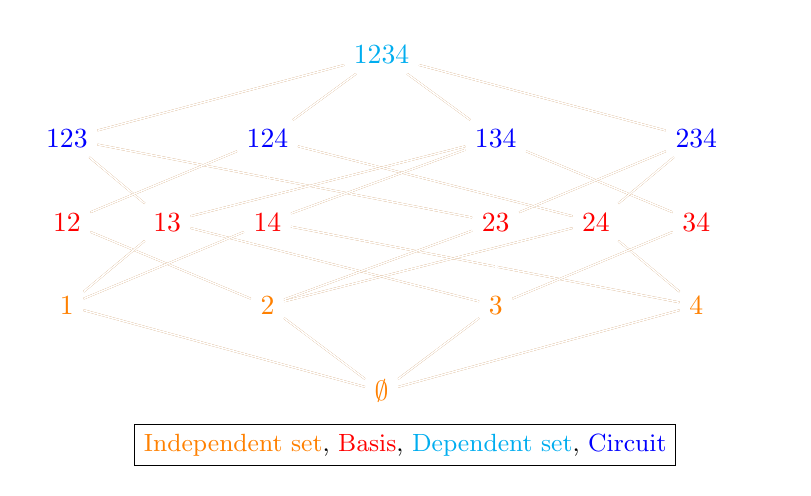
\begin{tikzpicture}

\matrix (a) [matrix of math nodes, column sep=0.6cm, row sep=0.6cm,]{
 & & &\textcolor{cyan}{
1234} & & & &\\
 \textcolor{blue}{
123}& &\textcolor{blue}{
124} & &\textcolor{blue}{
134} &  & \textcolor{blue}{
234}  \\
\textcolor{red}{12} & \textcolor{red}{13} & \textcolor{red}{14} & & \textcolor{red}{23} & \textcolor{red}{
24} & \textcolor{red}{
34} \\
\textcolor{orange}{1}& &\textcolor{orange}{2} & & \textcolor{orange}{3}& & \textcolor{orange}{4} \\
& & & \textcolor{orange}{\emptyset} &  & & \\
&&&&&& \\};

\foreach \i/\j in {1-4/2-1, 1-4/2-3, 1-4/2-5, 1-4/2-7, 2-1/3-1, 2-1/3-2, 2-1/3-5, 2-3/3-1, 2-3/3-3, 2-3/3-6, 2-5/3-2, 2-5/3-3, 2-5/3-7, 2-7/3-5, 2-7/3-6, 2-7/3-7, 3-1/4-1, 3-1/4-3, 3-2/4-1, 3-2/4-5, 3-3/4-1, 3-3/4-7, 3-5/4-3, 3-5/4-5, 3-6/4-3, 3-6/4-7, 3-7/4-7, 3-7/4-5, 4-1/5-4, 4-3/5-4, 4-5/5-4, 4-7/5-4}
\draw[double, line width = 0.005mm, color = brown] (a-\i) -- (a-\j);

\node[draw] at (0, -2.5){\small \textcolor{orange}{Independent set}, \textcolor{red}{Basis}, \textcolor{cyan}{Dependent set}, \textcolor{blue}{Circuit} };

\end{tikzpicture}
\end{center}
\caption{Representation of $U_{2,4}$}

\end{figure}

Suppose $U_{2,4}$ were $\mathbb{F}_2$-representable. Then there is some $A = \mat_{m \times 4}(\mathbb{F}_2)$, 

$$A = \begin{pmatrix}
    v_1 & v_2 & v_3 & v_4
\end{pmatrix}$$

so that $U_{2,4} \sim M[A]$. We have the following observation.

\begin{lemma}
\label{f2lema}
    Suppose a set of vectors $A = \{w_1, w_2, \cdots, w_r\} \subseteq \mathbb{F}_2^n$ is minimaly linarly dependent, that means that it is linarly dependent but any proper subset of it is linearly independent. Then $w_1 + w_2 + \cdots + w_r = 0$.
\end{lemma}

\begin{proof}
    Because $A$ is linearly dependent, there exists a set of scalars $\{a_1, a_2, \cdots, a_r\}\in \mathbb{F}_2$ not all zero such that
    
    $$\sum_{i=1}^r a_iv_i = 0.$$
    
    If for some $1\leq j \leq r$ we have $a_j = 0$ then we also have 
    
    $$\sum\limits_{\substack{i = 1 \\ i \neq j}} ^r a_iv_i = 0$$

    but not all out of $a_1, \cdots a_{j-1}, a_{j+1}, \cdots a_r$ are 0. This means that ${v_1, \cdots, v_{j-1}, v_{j+1}, \cdots, v_r}$ is linearly dependent, which is not true by assumption. Therefore, for all $1\leq j \leq r$ we have $a_j \neq 0$. But since the field is $\mathbb{F}_2$ this forces $a_j = 1$ for all $j$. Hence, we obtained what we want, namely

     $$\sum_{i=1}^r a_iv_i = 0 =  \sum_{i=1}^r 1 \cdot v_i = 0.$$
    
\end{proof}

If the matroid $U_{2,4} \sim M[A]$ for the above $A$ then we would have all of the three element subsets of vectors to be minimally linearly dependent. This means by lemma(\ref{f2lema}) that $v_1 + v_2 + v_3 = 0$ and $v_1 + v_2 + v_3 = 0$. However, we are in $\mathbb{F}_2$ so 


$$v_1 + v_2 + v_3 = 0 \iff v_1 + v_2 + (v_3 + v_3) = v_3 \iff v_1 + v_2 = v_3 $$

And in the same way $v_1 + v_2 = v_4$. This implies that
$$v_3 + v_4 = (v_1 + v_2 )+ (v_1 + v_2) = 0$$
so the set $\{v_3, v_4\}$ is linearly dependent, which is a contradiction. So $U_{2,4}$ is not $\mathbb{F}_2$-representable. However, $U_{2,4}$ is $\mathbb{F}_3$-representable. For instance the following matrix taken from \cite[20]{oxley1} works, namely

$$A = \begin{pmatrix}
    1 & 0 & 1 & 1 \\
    0 & 1 & 1 & 2
\end{pmatrix}$$.

 We see that no column vector of $A$ is 0, so all single-element subsets are independent. No vector is a scalar multiple of each other, so two element subsets are independent. Finally, no 3-element subsets can be independent, since the dimension of the $\mathbb{F}_3^2$ is 2, so the dimension of any subspace is at most 2.

To conclude the example of $U_{2,4}$, we will show that $U_{2,4}$ has an interesting property that it is not a graphic matroid. In other words, we can show that there is no graph $G$ such that $U_{2,4} \sim M$ where $M$ is the matroid formed by the set of edgs of $G$ with the usual rules. 

We will show $U_{2,4}$ is not graphic by contradiction, that is assume $U_{2,4}$ is graphic and let $G$ be the graph it represents. Then $G$ has four edges and since all two-element subsets of $U_{2,4}$ are independent we see that $G$ has no loops or parallel edges. In particular, all three-element subsets of $U_{2,4}$ are circuits, so in the graph the edges they correspond to form a cycle. But if both sets $\{1,2,3,\}$ and $\{1,2,4\}$ corresonds to edge cycles without parallel edegs it immediatly follows that $3$ and $4$ connect the same vertices, i.e. are parallel edges, which is a contradiction. It follows that $U_{2,4}$ is not graphic.

%In the succeeding sections, we will also consider an example of a matroid, which is not representable over any field.



\section{Graphic matroids}

TRYING TO DO GRAPHS, DONT LAUGH!!

\tikz \graph {A -> {b,c} -> }


\section{Algebraic matroids}

An interesting concept of independence arises in the study of field theory. We will present an interesting class of matroids derived from the concept of algebraic independence. For the rest of this section we will use the notation $\mathbb K / \mathbb F$ to refer to some field $\mathbb K$ and a subfield $\mathbb F$.

TODO: add example, prove transitivity.

\begin{defn}
  A subset $\{ s_1 \ldots s _n \} \subseteq \mathbb K / \mathbb F$ is said to be algebraically independent (over $\mathbb F$) if it doesn't satisfy any nontrivial polynomial with coefficients in $\mathbb{F} $, i.e.
  \begin{align*}
  \forall f \in F[X _1 \ldots X _n], \neg\left( f \neq  0 \land  f(s _1 \ldots s _n) = 0\right).
  \end{align*}
\end{defn}

Transcendental numbers are special cases of single element algebraically independent sets. Although it is well known that the complex numbers $e$ and $\pi$ are transcendental over $\mathbb{Q} $, it hasn't yet been proven that $\{e, \pi \}$ is algebraically independent.

We will now discuss the notion of algebraic dependence.

\begin{defn}
  Let $a \in \mathbb K / \mathbb F$ and $B = \{b _1 \ldots b _n \} \subseteq  \mathbb K / \mathbb F$. We say that $a$ is algebraically dependent on $B$ (over $ \mathbb{F} $) if $a$ is algebraic over $\mathbb F(b _1 \ldots b _n )$. Given some $A \subseteq  \mathbb K / \mathbb{F} $, we say that $A$ is algebraically dependent on $B$ (over $\mathbb{F} $) if every element of $A$ if algebraic on $B$ (over $\mathbb{F} $).
\end{defn}

\begin{lemma}\label{lem:algebraic-dependence-transitivity}
  Consider $A, B, C \in \mathbb K / \mathbb{F} $ such that $A$ is algebraic over $B$ and $B$ is algebraic over $C$. It then follows that $A$ is algebraic over $C$.
\end{lemma}

\begin{proof}
  TODO
\end{proof}

\begin{theorem}\label{thm:algebraic-matroids-are-matroids}
    Given a finite subset $E \subseteq \mathbb K / \mathbb F$, the pair $(E, \mathcal I)$  where $\mathcal I$ is the set of algebraically independent subsets of $E$ forms a matroid.
\end{theorem}

    Although~\cite{oxley1} offers a proof based on independent sets and the concept of algebraic dependence, we will instead present a proof based on the basis of our supposed matroid. The part focused on proving the exchange lemma is inspired by~\cite{milne2022}, although the rest will be a lot more simple (no need to involve Zorn's lemma) because we are working in a finite subset.


  We start by proving the following lemma:
  \begin{lemma}\label{lem:algebraic-indep-smaller-than-dep}
    Consider finite $A, B \subseteq \mathbb K / \mathbb F$, such that $A$ is independent over $\mathbb F$ and dependent on $B$ (over $\mathbb F$). Then $|B| \geq |A|$.
  \end{lemma}

  \begin{proof}
    We will prove the statement by induction on the number of elements in $A \setminus B$:
    \begin{enumerate}
      \item If $A \setminus B = \varnothing $ then $A \subseteq B$ and $|A| \leq |B|$ follows trivially.
      \item Assume the statemenet is true for some $|A \setminus B| = |A| - (k + 1)$ (where $k = |A \cap B$). We will attempt to prove it for $|A \setminus B| = |A| - k$. Let $a _1 \ldots a _n$ be the elements of $A$ such that $a _1 \ldots a_k$ are all the members of $A \cap B$ for some $k$. Let $ a _1 \ldots a_k, b _{k + 1} \ldots b _m$ be the elements of $B$. It remains to prove that $m \geq n$.

        As $a _{k + 1}$ is not dependent on $\{a _1 \ldots a_k\}$ but is dependent on $B = \{a _1 \ldots a _k, b _{k + 1} \ldots b_m\}$, there must exist some $k + 1 \leq j \leq m$ such that $a _{k + 1}$ is dependent on $\{a _1 \ldots a _k, b _{k + 1} \ldots b_j\}$ but  not on $\{a _1 \ldots a _k, b _{k + 1} \ldots b _{j - 1}\}$. Because $a _{k + 1}$ is dependent on $\{a _1 \ldots a _k, b _{k + 1} \ldots b_j\}$, we know there exists some polynomial $f \in \mathbb F[x _1 \ldots x _{j + 1}]$ such that 
        \begin{align*}
           f(a _1 \ldots a _{k}, b _{k + 1} \ldots b _{j}, X) \neq  0 \land 
           f(a _1 \ldots a _{k}, b _{k + 1} \ldots b _{j}, a _{k + 1})  = 0.
        \end{align*}

      We can write $f$ as
      \begin{align*}
        f(x _1 \ldots x _{j + 1}) 
        = \sum_i f _i(x _1 \ldots x _{j - 1}, x _{j + 1}) x _j ^i.
      \end{align*}

        We know that $f(a _1 \ldots a _{k}, b _{k + 1} \ldots b _{j}, X) \neq  0$, therefore at least one of $f _i \neq 0$. Let $g = f _i $ such that $f _i \neq 0$. Because $a _{j + 1}$ is not algebraic over $\{a _1 \ldots a _k, b _{k + 1} \ldots b _{j - 1}\}$, we know that 
        \begin{align*}
          g(a _1 \ldots a _k, b _{k + 1} \ldots b _{j - 1}, a _{k + 1}) \neq 0.
        \end{align*}

        This implies that $f(a _1 \ldots a _k, b _{k + 1} \ldots b _{j - 1}, X, a _{k + 1}) \neq 0$. Since $ f(a _1 \ldots a _{k}, b _{k + 1} \ldots b _{j}, a _{k + 1})  = 0$, we can conclude that $b_j$ is algebraic over $\{a _1 \ldots a _{k + 1}, b _{k + 2} \ldots b _j\}$.

        Construct $B' = B + a _{k + 1} - b_j$. Having proven that $b_j$ is dependent on a subset of $B'$, it is also dependent on $B'$. All other elements of $B$ are also dependent on $B'$ (because any variable is algebraic over a field extension it generates, i.e. $t$ is algebraic over $\mathbb F(t)$). We recall that $A$ is dependent on $B$, so by the transitivity of algebraic dependence (lemma (\ref{lem:algebraic-dependence-transitivity})), we know that $A$ is algebraic over $B'$. We also notice that $A$ and $B'$ have $k + 1$ elements in common, therefore the statement is proven by the induction hypothesis.
    \end{enumerate}
  \end{proof}

We will now show that all basis in our supposed matroid have equal cardinality.

\begin{lemma}\label{lem:algebraic-matroid-equal-size-basis}
  Given some finite subset $E \subseteq \mathbb K / \mathbb F$, maximal independent subsets of $E$ (in the partially ordered set induced by inclusion) have equal cardinality.
\end{lemma}

\begin{proof}
  Let $A$ and $B$ be maximal independent subsets of $E$. If both sets are $\varnothing$, then our proof is done. If one set is $\varnothing$ and one isn't, we clearly have a contradiction, as $\varnothing$ is a strict subset of the other set, hence not maximal. We therefore assume the existence of some $a \in A$ and $b \in B$. 

  We know that $A$ is maximal, therefore any $b \in B$ is algebraically dependent on $A$. We can therefore conclude that $B$ is algebraically dependent over $B$. We recall that $B$ is also independent, which means we can use lemma (\ref{lem:algebraic-indep-smaller-than-dep}) to prove that $|A| \geq |B|$. We can apply a similar argument to show that $|B| \geq |A|$, which together with our previous statement shows that $|A| = |B|$, proving the lemma.
\end{proof}

\begin{proof}[Proof of theorem (\ref{thm:algebraic-matroids-are-matroids})]
    We will construct the matroid using the basis definition. We need to first show that at least one exists, and then show that the exchange property holds.

  We consider the partially ordered set of independent subsets of $E$ ordered by inclusion. We notice that $ \varnothing $ is independent (as the only polynomial of $0$ variables which can be satisfied by $\varnothing $ is the trivial polynomial). Any finite nonempty partially ordered set has at least one maximal element, so a basis exists.

  It now remains to prove the exchange property. That is, given two basis $A, B \subseteq \mathcal B$ and some $a \in A \setminus B$, we can find some $b \in B \setminus A$ such that $B - b + a \in \mathcal B$. Let $n = |A| = |B|$ (we know the two basis have equal cardinality from lemma (\ref{lem:algebraic-matroid-equal-size-basis})). Assume the statement is not true. That is, all $b _i \in B$ are dependent on $A - a$, which means $B$ is dependent on $A - a$. It follows from lemma (\ref{lem:algebraic-indep-smaller-than-dep}) that $|B| \leq |A - a|$, which is equivalent to $n \geq n - 1$, hence a contradiction.
\end{proof}


\section{Dual Matroids}
The concept of \textit{duality} is an interesting feature of matroid theory. It helps to extend some of the constructions in our prototypical examples in representable and graphic matroids, such as the notion of orthogonality in vector spaces and the concept of a planar dual of a plane graph, to general matroids. In this section we will introduce the definitions and  properties of dual matroids.

%Before starting with the formal definitions, porperties and theorems is important that we state the most important concept of this chapter, that is, similar to the chapter name, the concept of a \textit{dual}, or more precisely, the \textit{dual of a matroid}.\\

% I DONT THING THE ABOVE PARAGRAPH ADDS ANY CONTENT

If we have a matroid $M$, with sets $(E,B)$, or in other words $M$ is a matroid on $E$ with $B$ as its collection of bases. Then its dual will refer to a different and new matroid, which we denote by $M*$. This new matroid has the property that it is "related" to the original matroid, so it has the same ground set $E$ of the original matroid $M$, but a different basis set, this new basis collection will be called $B*$, so this gives us that $M*$ will be defined by the following pair of sets $(E,B*)$. Where $B^*$ will a set such that is is the complement of the bases set $B$ in $M$, which implies that, the bases set of $M$ and $M^*$ will be always disjoint.

This can be seen more clearly in the following digram:
\begin{figure}[H]
    \centering
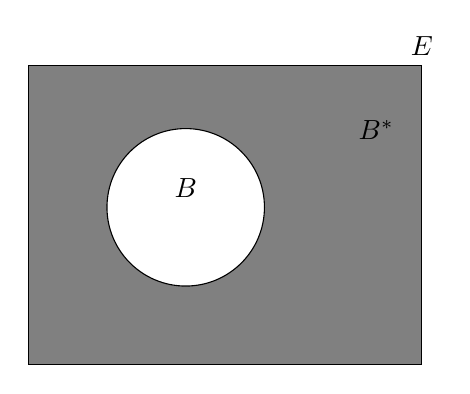
\begin{tikzpicture}
        \filldraw[fill=gray] (-2,-2) rectangle (3,1.8) node [text=black,above] {$E$} node at (19:3) [text= black, left = 2pt] {$B^*$};
        \scope % B
        \clip (0,0) circle (1);
        \fill[white] (0,0) circle (1.5);
        \endscope
        \draw (0,0) circle (1) node [text=black,above] {$B$};
\end{tikzpicture}
\caption{Venn diagram showing, B the basis set of $M$, and $B^*$ the basis set of $M^*$}%
\label{graphic}%
\end{figure}

We also have the depiction from previous sections, but know we will also the one that will correspond to the dual on this specific case. To the \textbf{left} we have the depiction corresponding to the \textbf{original matroid}, and to the \textbf{rigth} we have the one corresponding to its \textbf{dual matroid}. 
Notice how the ground set will be composed of 4 components $E=\{1,2,3,4\}$, and in the original matroid has bases $12$ and $23$, in red. So, its dual has bases $34$ and $14$, respectively, also in red but in the rigth-side diagram. This is because, the complement of the elements $12$ is $34$, and the complement of $23$ is $14$.


\begin{tikzpicture}[H]
\centering
\matrix (a) [matrix of math nodes, column sep=0.3cm, row sep=0.6cm,]{
 & & &\textcolor{cyan}{
1234} & & & &\\
 \textcolor{cyan}{
123}& &\textcolor{cyan}{
124} & &\textcolor{cyan}{
134} &  & \textcolor{cyan}{
234}  \\
\textcolor{red}{12} & \textcolor{blue}{13} & \textcolor{cyan}{14} & & \textcolor{red}{23} & \textcolor{cyan}{
24} & \textcolor{cyan}{
34} \\
\textcolor{orange}{1}& &\textcolor{orange}{2} & & \textcolor{orange}{3}& & \textcolor{blue}{4} \\
& & & \textcolor{orange}{\emptyset} &  & & \\
&&&&&& \\};

\foreach \i/\j in {1-4/2-1, 1-4/2-3, 1-4/2-5, 1-4/2-7, 2-1/3-1, 2-1/3-2, 2-1/3-5, 2-3/3-1, 2-3/3-3, 2-3/3-6, 2-5/3-2, 2-5/3-3, 2-5/3-7, 2-7/3-5, 2-7/3-6, 2-7/3-7, 3-1/4-1, 3-1/4-3, 3-2/4-1, 3-2/4-5, 3-3/4-1, 3-3/4-7, 3-5/4-3, 3-5/4-5, 3-6/4-3, 3-6/4-7, 3-7/4-7, 3-7/4-5, 4-1/5-4, 4-3/5-4, 4-5/5-4, 4-7/5-4}
\draw[double, line width = 0.005mm, color = brown] (a-\i) -- (a-\j);

\end{tikzpicture}
\begin{tikzpicture}[H]
\centering
\matrix (a) [matrix of math nodes, column sep=0.3cm, row sep=0.6cm,]{
 & & &\textcolor{cyan}{
1234} & & & &\\
 \textcolor{cyan}{
123}& &\textcolor{cyan}{
124} & &\textcolor{cyan}{
134} &  & \textcolor{cyan}{
234}  \\
\textcolor{cyan}{12} & \textcolor{blue}{13} & \textcolor{red}{14} & & \textcolor{cyan}{23} & \textcolor{cyan}{
24} & \textcolor{red}{
34} \\
\textcolor{orange}{1}& &\textcolor{blue}{2} & & \textcolor{orange}{3}& & \textcolor{orange}{4} \\
& & & \textcolor{orange}{\emptyset} &  & & \\
&&&&&& \\};

\foreach \i/\j in {1-4/2-1, 1-4/2-3, 1-4/2-5, 1-4/2-7, 2-1/3-1, 2-1/3-2, 2-1/3-5, 2-3/3-1, 2-3/3-3, 2-3/3-6, 2-5/3-2, 2-5/3-3, 2-5/3-7, 2-7/3-5, 2-7/3-6, 2-7/3-7, 3-1/4-1, 3-1/4-3, 3-2/4-1, 3-2/4-5, 3-3/4-1, 3-3/4-7, 3-5/4-3, 3-5/4-5, 3-6/4-3, 3-6/4-7, 3-7/4-7, 3-7/4-5, 4-1/5-4, 4-3/5-4, 4-5/5-4, 4-7/5-4}
\draw[double, line width = 0.005mm, color = brown] (a-\i) -- (a-\j);
\end{tikzpicture}

\begin{center}
\begin{tikzpicture}[H]
\centering
\node[draw] at (0, -2.5){\small \textcolor{orange}{Independent set}, \textcolor{red}{Basis}, \textcolor{blue}{Circuit}, \textcolor{cyan}{Dependent set}}
\end{tikzpicture}
\end{center}




We know that the basis set of a matroid is obtained from its set of independet sets $I$.
Using this diagrams we highligth an idea that will be useful later in this chapter.
This is, that the basis set of a matroid is given by a subset of $E$, the remaing elements in $E$ that are not in de basis if added to the basis will be linearly dependent, but also we can take any remaining element of $E$ and exchange it with an element in the basis and we will have another basis for $E$. With this intuition in mind, we can continue with a theorem.


To formalize the definition of $B^*$ we have the following:
\begin{theorem}
    Let $M$ be a matroid given by $(E,B)$, and B*$(M)$ be $\{E(M) - B:B\in B(M)\}$. Then B*$(M)$ is the set of bases of a matroid on $E(M)$
\end{theorem}

Or in other words, B* is the set of all the complement independent bases of $B$. Then we can give the following definition.

\begin{defn}
    Let M be a matroid with the pair (E,B), given B* as defined above, the new matroid M*=(E,B*) is the dual of M.
\end{defn}

In the theorem we say that B*$(M)$ is the set of bases of a matroid on $E(M)$, but this is not be trivially clear, so we need to prove it.

However to prove it we will mahe use of the following result, that comes from our properties of the basis set B of our matroid M in Section 2.2

Lemma. The set $B$ of bases of a matroid M has the following property:
$(B2)^*$ If $B_1$ and $B_2$ are in B and $x \in B_2 - B_1$,then there is exist and element $y$ of $B_1 - B_2$ such that $(B_1 - y) \cup x \in B$

\textit{For comparison this was the original (B2): \\
$(B2)$ If $B_1,B_2\in\mathcal{B}$ and $x\in B_1 - B_2$, then there exists a $y\in B_2 - B_1$ such that $(B_1 - x)\cup y \in\mathcal{B}$.}\\

First we will prove $(B2)^*$:
\begin{proof}
  We note that $B_1$ is by definition a base, this means that if we add a new element in the ground set to it, it will become a minimal dependet set, in other words $B_1 \cup x$ contains a unique circuit $C_1 \in C$. Since we have $C_1$ a dependent set and $B_2$ another base, and thus independet, then $C_1 - B_2$ will be non-empty, so there exists and element $y$ such that $y \in C_1 - B_2$, but as $C_1$ is the circuit created from $B_1 \cup x$, then $y \in (B_1 \cup x) - B_2$, but as $x \neq y$, then $y \in B_1 - B_2$. Now, lets take $B_1 - y$, this will not be a basis, but it will be an independent set, if now we take $(B_1 - y)\cup x$, this will clearly not contain the circuit $C_1$, since this was the unique circuit generated from $B_1 \cup x$, so the set $(B_1 - y)\cup x$ must be independent. Finally, we observe that $(B_1 - y)\cup x$ implies that we add and elemnts to the set and we take out one element to the set, so the cardinality will remain equal, that is: $|(B_1 - y)\cup x|=|B_1|$.
As we have that $(B_1 - y)\cup x$ is and independent set and has the same cardinality as the the base $B_1$, then by definition $(B_1 - y)\cup x$ is also a base.  
\end{proof}

Now, we prove that $B^*(M)$ is the set of a base of a matroid on $E(M)$
\begin{proof}
    As $B(M)$ is non-empty, $B^*(M)$ is non-empty, hence, the property $(B_1)$ holds for $B^*(M)$. 
    Now, consider two members of $B^*(M)$, $B^*_1$ and $B^*_2$, not equal such that there exists an element $x \in (B^*_1 - B^*_2)$. Let, $B_1 = E - B^*_1$ and $B_2 = E - B^*_2$. We can see that $B^*_1 - B^*_2 = B_2 - B_1$, thus $x \in B_2 - B_1$. By $(B2)^*$, there exists and element $y \in  B_1 - B_2$ such that $(B_1 - y)\cup x$ is a base of $M$, but observe that $B_1 - B_2 = B^*_2 - B^*_1$, hence this is the same as saying that there exists and element $y \in  B^*_2 - B^*_1$ such that $(B_1 - y)\cup x$ is a base of $M$. Hence, by definition of dual, $E-((B_1 - y)\cup x) \in B^*(M)$. But, $E-((B_1 - y)\cup x) = ((E-B_1)-x)\cup y) = (B_1^* - x)\cup y$, which is in the family $B^*$. Thus, $B^*(M)$ satisfes $(B2)$. As $B^*(M)$ satisfies properties $(B1)$ and $(B2)$, this is indeed the set of bases of a matroid on $E$.
\end{proof}

The matroid M*, is the dual of M. Note that by the way is defined, and thanks to the proof above we see that $B(M^*)=B^*(M)$, moreover, due the nature that the definition of dual has, this is, that is the complement of the basis set, we have that
\begin{itemize}
    \item \textit{The dual of the dual of a matroid M is the matroid M itself, $i.e., (M^*)^* = M$}
\end{itemize}
This is because if we take the complement $B^*$ of the basis set $B$, and then we take this complement $B^*$ and take its complement once again, we will return to the original set $B$, or in other words: If $E-(E - B) = B$.\\

As an example, let $U_{k,n}$, be a k-uniform matroid. We know that its bases will be all the k-element subsets of $E(U_{k,n})$, we know that this matroid is defined over a set of $n$ elements, and its basis has exactly $k$ elements, hence the bases of $U_{k,n}$* are be all $(n-k)-element$ subsets of the ground set, as this will be the complement of the basis set of $U_{k,n}$. This is equal to saying that the dual of the matroid $U_{k,n}$ is given by $U_{k,n}$* $= U_{n-k,n}$\\


Now that we have introduced duals is useful to give some additional notation. That is, given a matroid $M$ with a dual $M^*$, the \textit{bases} of the matroid $M^*$ are called \textit{cobases} of $M$. Similarly, the \textit{independent sets} of $M^*$ are called \textit{coindependent sets} of $M$, the circuits of $M^*$ are called \textit{cocircuits} of $M$, \textit{hyperplanes} are called \textit{cohyperplanes}, and the \textit{spanning sets} are called \textit{cospanning sets} of $M$ and so on.\\

This leads us to some elemenary relationships between these sets. 

$Proposition:$ Let M be a matroid in a set E and suppose $X \subseteq E$. Then,
    \begin{enumerate}
        \item $X$ is independent if and only if $E-X$ is cospanning.

        \item $X$ is spanning if and only if $E-X$ is coindependent.

        \item $X$ is a hyperplane if and only if $E-X$ is a cocircuit

        \item $X$ is a circuit if and only if $E-X$ is a cohyperplane.
    \end{enumerate}

\begin{proof}
    All of the proofs follow directly from the definitions. [We will prove a) and b)]

    a) Suppose $X$ is independent. This means there exists a basis $B \in \mathcal{B}(M)$ so that $X \subset B$. Because $X \subset B \subset E$ and the operation of taking complements is "inclusion reversing" we have $E-B \subset E - X$. Verifying directly, if $x \in E - B$ this means $x \in E$ and $x \notin B$. Because $X \subset B$ this implies that $x \in E$ and $x \notin X$ so by definition $x \in E - X$ and the conclusion follows. Because $E - B$ is a cobasis and $E - X$ is a set containing a cobasis, then it is a cospanning by definion.

    Similarly if $E - X$ is cospanning then it contains a cobasis which is by definition of the form $E - B$ for some $B \in \mathcal{B}(M)$. By the analagous reasoning as for the forward direction $E - B \subset E - X$ implies $X \subset B$. That is because if $x \in X$ then $x \notin E - X$ and $x \notin X - B$. This means $x \in B$ concluding $X \in B$. Since $B$ is an independent set then $X$ is independent set as well, we are done.

    b) Same as a). A set $X\subset E$ being spanning implies it contains a $B \in \mathcal{B}(M)$. So  $B \susbet X$ which implies $E - X \subset E - B$. Because $E - B$ is cobasis by definition, any of its subsets are coindependent. 

    If $E - X$ is coindependent, it is contained in a cobasis, so by definition there exists a $B \in \mathcal{B}$ so that $E - X \subset E - B$. As before this implies that $B \subset X$ and $X$ is spanning.

    c)  If $X$ is a hyperplane, then $X$ is not spanning but for all $y \in E - X$ we have $X \cup y$ is spanning, which means there is for every such $y$ a basis $B_y \in \mathcal{B}$ so that $B_y \subset X \cup y $. By b) we know that $X$ is not spanning implies $E - X$ is not coindependent. But for any $z \in E - X$ we have $(E-X)-z = E - (X \cup z)$ is coindependent because $X \cup z$ is spanning. So $E - X$ is a cocircuit by definition.

    Conversly, if $E - X$ is a cocirucuit, then $E-X$ is not coindependent but for all $x \in E - X$ we have $(E - X) - x$ = $E - (X \cup x)$ is coindependent. By b) this means that $X$ is not spanning but for all $x \in E-X$, we have $X \cup x$ is spanning, so $X$ is a hyperplane.

    d) Same as things before.
\end{proof}\\

Similar to the case with the bases and cobases, the rank function of the dual matroid is usually denoted by $r^*$, and is normally referred as the $corank$ $function$ of $M$. Using the definition of bases of the dual matroid, this is, that is build with the complement bases of the set of the orginal matroid, as well as the fact that matroid and its dual are both on the same ground set, we have the following:

\begin{itemize}
    \item $r(M) + r$*$(M) = |E(M)|=|E(M^*)|$
\end{itemize}

And in fact, we can generalize this to obtain an explicit formula for the for the corank function of the matroid. 

For all subsets X of the ground set E of a Matroid M,
\begin{itemize}
    \item $r^*(X)=r(E-X)+|X|-r(M)$
\end{itemize}

\begin{proof}
    Let $I^*$ be a independet subset of $X$ in $M^*$, such that it is not a subset of some other set in $X$, this is $r^*(X)=|I^*|$. Similarly, let $I$ be a independent subset of $E-X$ in $M$, such that it is not a subset of some other set in $E-X$, this is $r(E-X)=|I|$. And let $B$ be an independent subset of $E-I^*$, such that it is not a subset of some other set in $E-I^*$ and contains $I$. Since, this are independent subsets that are not subsets of any other element in their respective sets, then we have $r(B)=r(E-I^*)$ and $r(E-I^*)=r(M)$, and hence $B$ is a base of M.
    Now, let $B^*=E-B$, since $B$ is a base of $M$, by definition $B$ is a base of $M^*$. We can onserve that $I^*\subseteq B^*$ and  $B^*\cap X=I^*$. Similarly, $I\subseteq B$ and  $B\cap (E-X)=I$. In particular we see that, $|B\cap X|=|B|-|I|$, thus
    $|X|=|X\cap B|+|X\cap B^*|=|B|-|I|+|I^*|=r(M)-r(E-X)+r^*(X)$
\end{proof}


%Subsection
Now we will talk about duals of representble matroids.
Let A be an $m \times n$ matrix over the field $F$, and let M be vector matroid $M[A]$ of $A$. Then we have that the groud set of $M$ is the set $E$ of column labels of $A$. Note that, in general, $M[A]$ does note uniquely determine $A$. Furthermore, M remains unchanged if we perform any of the following operarations on $A$, which include the \textit{elementary row operations} seen in the linear algebra courses.
\begin{enumerate}
    \item Interchange two rows.
    \item Multiply a row by a non-zero member of $\mathbb{F}$.
    \item Replace a row by the sumof that row with another row.
    \item Adjoin or remove a zero row.
    \item Interchanging two columns (the labels moving with the columns).
    \item Multiply a column by a non-zero member of $\mathbb{F}$.
\end{enumerate}

The reason for this is because when constructiong the matroid $M$ form a matrix $A$, we only care about the independence (or dependence) that each column vector in the matrix has with one another. So, as long as the independence and dependece between this is keep the same, the values inside the columns are not relevant.

Assume that the matrix A is non-zero. It is known that by using the operations previusly mentioned A can be reduced to be of the form $[I_r|D]$, where $I_r$ is the $r \times r$ identity matrix and $D$ is some $r \times (n-r)$ matrix over $F$. We can clearly see that $r(M)=r$ (the dimension fo the identity matrix). 

Suppose that the columns of $[I_r|D]$ are labelled, in order, in the following form, $e_1, e_2,...,e_n$. This will be the ground set $E=\{e_1, e_2,...,e_n\}$. Then, we see that $\{e_1, e_2,...,e_r\}$ is a basis $B$ of $M$, once agina due to the dimesion of the identity matrix. We also label both, the rows and colums of $D$, in the following form, for the rows from top to bottom, $e_1, e_2,...,e_r$ and for the columns,  $e_{r+1}, e_{r+2},...,e_n$. This way to represent $M[A]$ can be seen more clearly in the following figure. We will refer to both $[I_r|D]$ and $D$ as the \textit{standard representative matrices} for $M$, \textit{with respect to $\{e_1, e_2,...,e_r\}$}. Similarly, we use \textit{reduced standard representative matrix} if we want to refer only to $D$.

\begin{figure}[H]
    \centering
    \includegraphics{SRF.png}
    \caption{Standard representative matrices for M. [3]}
    \label{fig:enter-label}
\end{figure}
Note that, in the figure, in $[I_r|D]$ only the columns are labelled, but in $D$, both the rows and columns ae labeled.

We can now use this construction to determine the dual of a vector matroid using the following theorem.

\begin{theorem}
    Let M be the vector matroid of the matrix $[I_r|D]$ where the columns of this matrix are labelled, in order, $e_1, e_2,...,e_n$ and $1\leq r< n$. Then $M^*$ is the vector matroid of $[-D^T|I_{n-r}]$ where its columns are also labelled $e_1, e_2,...,e_n$ in that order.
\end{theorem}

\begin{proof}
    We assume that $[I_r|D]$ is as in the contruction of the theorem above. Then $[-D^T|I_{n-r}]$ is as follows


    Let $B$ be a basis of $M$. We need to show that $E-B$ is a basis of the vector matroid of $[-D^T|I_{n-r}]$. We can rearrege the columns of $[-D^T|I_{n-r}]$, such that $B=\{e_1,\dots,e_s, e_{r+1}, \dots , e_{r+(r-s)}$, for some $s \leq r$. This is possible becasue we know that it does not affect the corresponding matroid, so the only change it bring to rearrange rows and columns of $[I_r|D]$ is the re-arrenge of columns and rows of $[-D^T|I_{n-r}]$. 
    
    Using this we can partition $[I_r|D]$ in the following form
    \begin{figure}[H]
    $$\begin{bmatrix}
    I_s & 0 & D_{11} & D_{12\\
    0 & I_{r-s} & D_21 & D_22\\
    \end{bmatrix}
    % 
    \rightarrow
    \begin{bmatrix}
    -D_{11}^T & -D_{21}^T & I_{r-s} & 0\\
    -D_{12}^T & -D_{22}^T & 0 & I_{n-(2r-s)}\\
    \end{bmatrix}$$
    \end{figure}
    First, lets analyse the partition of $[I_r|D]$.
    Here me made the partition such that the first component $I_s$ has columns from $(e_1 \dots e_s)$. $I_{r-s}$ has columns from $(e_{s+1} \dots e_r)$, $D_11$ and $D_21$ have from $(e_{r+1} \dots e_{2r-s})$, and finally $D_12$ and $D_22$ have from $(e_{(2r-s)+1} \dots e_n)$.
    
    We have that $B$ is a base, this means that it must have the same size as $I_r$. Due to the way the matrix $[I_r|D]$ is partitioned, that is, if the we take the components in the partirion that contain the columns of the basis we have the following matrix:
    \begin{figure}[H]
        \centering
        $$\begin{bmatrix}
        I_s & D_{11}\\
        0 & D_{21}\\
        \end{bmatrix}$$
    \end{figure}
    As this matrix has the components that contain all the elements in the basis implies that it must have $rank = r$ (the rank of $[I_r|D]$), but here $I_s$ has $rank = s$, as it is the identity matrix. Hence, the the rank of $D_11$ is $r-s$, which also corresponds to the rank of $D_21^T$.
    
    If we now observe the partition of $[-D^T|I_{n-r}]$, this will gave the same partition lengths in each component as the ones mentioned for $[I_r|D]$ above. 
    
    in the rigth side, we notice that following a similar reasoning this will have a rank of $n-(2r-s)$    
\end{proof}

By convention the form $[−D^T |I_{n−r}]$ instead of $[D^T |I_{n−r}]$. However it is important to remark that this does not bring any problem, because, as we previusly stated, the use of \textit{elementary row operations} does not affect the matroid of a matrix. 

From the previous theorem a remarkable result follows almost directly. 
\begin{itemize}
    \item  \textbf{Corollary 1. :} If a matroid \textit{M} is \textit{representable} over a field $\mathbb{F}$, then \textit{M*} is also representable over the same field $\mathbb{F}$.
\end{itemize}


$Example:$ Consider the vector matroid $M$ with the following representation over $R$
        \begin{figure}[H]
            $$A = \begin{bmatrix}
                1 & 0 & 0 & 1 & 0 & 1 \\
                0 & 1 & 0 & 1 & -1 & 0 \\
                0 & 0 & 1 & 0 & 1 & 1 \\
            \end{bmatrix}$$
        \end{figure}
        
The by the theorem the corresponding dual matroid $M^*$ is the vector matroid represented by 
        \begin{figure}[H]
            $$A^* = \begin{bmatrix}
                -1 & -1 & 0 & 1 & 0 & 0 \\
                0 & 1 & -1 & 0 & 1 & 0 \\
                -1 & 0 & -1 & 0 & 0 & 1 \\
            \end{bmatrix}$$
        \end{figure}
As and interesting note, this vector matroid $A$ is associated to the graph $K_4$ 
       \begin{figure}[H]
        \centering
            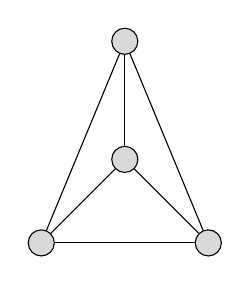
\begin{tikzpicture}[
                node distance = 15mm and 15mm,
                V/.style = {circle, draw, fill=gray!30},
                every edge quotes/.style = {auto, font=\footnotesize, sloped}
                    ]
                \begin{scope}[nodes=V]
                \node (1) {}; 
                \node (2) [below of=1] {}; 
                \node (3) [below left of=2] {}; 
                \node (4) [below right of=2] {}; 
                \end{scope}
                \draw (1) to (2); 
                \draw (1) to (3);
                \draw (1) to (4); 
                \draw (2) to (3);
                \draw (2) to (4); 
                \draw (3) to (4);
            \end{tikzpicture}
            \caption{$K_4$, the complete graph on 4 vertices}
            \label{fig:enter-label}
        \end{figure}

Aditionally, from this we can also verify the $rank$ and $corank$ propositions established before. This is, we can clearly observe that $A$ has a ground set $E=\{e_1, e_2, \dots , e_6\}$ with 6 elements, where each $e_i; i =1,2, \dots,6$ represents a column, hence $|E|=6$. We also see that $A$ has rank $r(A)=3$, which can be easily verified by observing the first 3 columns that correspond to the identity matrix in the construction of the form $[I_r|D]$. Similarly, if we observe the dual we notice that also $r(A^*)=3$. \\So, $r(A)+r(A^*)= 3 + 3 = 6 = |E|$\\


%

We have seen many concepts related to dual matroids, including some representations for vector matroids, however we have not gone that much into detail with graphic matroids. So, the reader could still be wondering, \textit{"Is it possible to have a graphic matroid whose dual is not grahic?"}

To answer that we have the following theorem

\begin{theorem}
    \item  The dual of a graphic matroid is itself graphic if and only if the underlying graph is planar.
\end{theorem}

\begin{proof}
    TODO
    Hello
\end{proof}



$Example:$ Let us consider the bipartite graph $K_{3,3}$.
\begin{figure}[H]
\centering
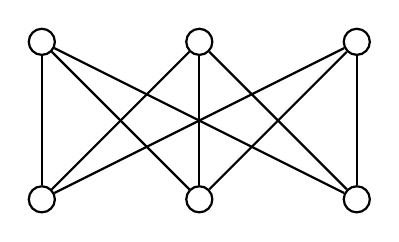
\begin{tikzpicture}[node distance={20mm}, thick, main/.style = {draw, circle}] 
    \node[main] (1) {}; 
    \node[main] (2) [below of=1] {}; 
    \node[main] (3) [right of=1] {}; 
    \node[main] (4) [below of=3] {}; 
    \node[main] (5) [right of=3] {}; 
    \node[main] (6) [below of=5] {}; 
    \draw (1) to (2); 
    \draw (1) to (4);
    \draw (1) to (6); 
    \draw (3) to (2);
    \draw (3) to (4); 
    \draw (3) to (6);
    \draw (5) to (2); 
    \draw (5) to (4);
    \draw (5) to (6);
    \end{tikzpicture}
    \caption{The bipartite graph $K_{3,3}$}
    \label{fig:enter-label}
\end{figure}

We can see it has 9 edges, so the ground set is $E=\{1,2,3, \dots, 9\} $.

\begin{figure}[H]
The matrix associated to the matroid $M(K_{3,3})$ is the following:
$$J = \begin{bmatrix}
    1 & 0 & 0 & 0 & 0 & 1 & 0 & 0 & 1\\
    0 & 1 & 0 & 0 & 0 & 1 & 1 & 0 & 1\\
    0 & 0 & 1 & 0 & 0 & 1 & 1 & 1 & 1\\
    0 & 0 & 0 & 1 & 0 & 0 & 1 & 1 & 1\\
    0 & 0 & 0 & 0 & 1 & 0 & 0 & 1 & 1\\
\end{bmatrix}$$
\end{figure}

This is because if we label the columns of $J$ as $E = \{e_1,\dots, e_9\}$ and define a matroid $M(J)$ on $E$, it is easy to see that we associate each column of $J$ to the correspondingly labeled edge in $K_{3,3}$, so that they generate the same matroid. Moreover, this means that we can take a basis for the column space of $J$, such as, $B = \{e_1, e_2, e_3, e_4, e_5\}$, such that it corresponds to a spanning tree $T$ of $K_{3,3}$ (See Figure 8.). In other words, this means that adding any other column to $J$ gives a linear dependency, more precisely a circuit in $M(J)$, and adding any edge to $T$ generates a cycle.
\begin{figure}[H]
    \centering
    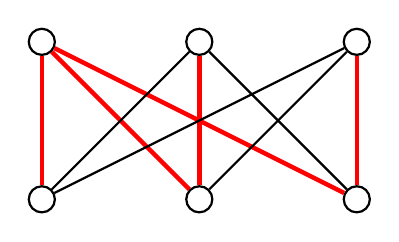
\begin{tikzpicture}[node distance={20mm}, thick, main/.style = {draw, circle}] 
        \node[main] (1) {}; 
        \node[main] (2) [below of=1] {}; 
        \node[main] (3) [right of=1] {}; 
        \node[main] (4) [below of=3] {}; 
        \node[main] (5) [right of=3] {}; 
        \node[main] (6) [below of=5] {}; 
        \draw [ultra thick,red] (1) to (2); 
        \draw [ultra thick,red] (1) to (4);
        \draw [ultra thick,red] (1) to (6); 
        \draw (3) to (2);
        \draw [ultra thick,red] (3) to (4); 
        \draw (3) to (6);
        \draw (5) to (2); 
        \draw (5) to (4);
        \draw [ultra thick,red] (5) to (6);
    \end{tikzpicture}
    \caption{Graph $K_{3,3}$, showing in red an example of edges that form a spanning tree, that can be associated accordingly to the basis of $J$.}
    \label{fig:enter-label}
\end{figure}

Now that we have show that $K_{3,3}$ has an associated matrix, which produces the same Matroid, we can use the Theorem 12. to obtain the corresponding dual. 
So we get, 
\begin{figure}[H]
  $$J^*=\begin{bmatrix} 
1 & 1 & 1 & 0 & 0 & 1 & 0 & 0 & 0\\
0 & 1 & 1 & 1 & 0 & 0 & 1 & 0 & 0\\
0 & 0 & 1 & 1 & 1 & 0 & 0 & 1 & 0\\
1 & 1 & 1 & 1 & 1 & 0 & 0 & 0 & 1\\
\end{bmatrix}$$
\end{figure}

As a sanity check we can see that;
$r(J) = 5$;  $r^*(J)=4$, and $|E(M)|=9$
Hence, we see that $r(M) + r^*(M) = |E(M)|$ holds.
According to the \textbf{Corollary 1.}, \textit{If a matroid \textit{M} is \textit{representable} over a field $\mathbb{F}$, then \textit{M*} is also representable over $\mathbb{F}$} , here we see that, both matroids are vector matroids over the field $\mathbb{F}_2$. 
Finally, in this example we can observe that $K_{3,3}$ is not a planar graph, this implies that, although $M(K_{3,3})$ is a graphic matroid, its dual, $M^*(K_{3,3})$ is not graphic.



\nocite{*} 
\bibliographystyle{abbrv}
\bibliography{sources}


\end{document}
